\chapter[Introduction]{Introduction\protect\footnote{This chapter has been accepted for publication at Journal of Physical Chemistry C in the form of a review article as Graphene: From Solid Support for Nucleobase Assisted Self-Assemblies to Functional Material for DNA Sequencing}}

Graphene, a two-dimensional atomistically thin allotrope of carbon, has attracted significant attention from the scientific community following the first unambiguous demonstration of the isolation of monolayer graphene by Andre Geim and Kostya Novoselov at the University of Manchester in 2004\supercite{geim_rise_2007, geim_graphene_2009}. The specific arrangement of carbon atoms in the graphene lattice leads to interesting physical, chemical and electrical properties, which multiple groups have exploited for applications in a broad spectrum of domains\supercite{berman_few_2013,chen_oxidation_2011, cui_cautionary_2017, su_impermeable_2014, berry_impermeability_2013, hayatdavoudi_mechanistic_2017} ranging from electronics\supercite{moreno_bottom-up_2018, fan_graphene_2019,sun_graphene_2010, kim_graphene-contact_2012, avouris_graphene_2010, baeumer_ferroelectrically_2015, bao_atomic-layer_2009,blake_graphene-based_2008, trung_graphene_2022,wang_transparent_2008, liu_ultratransparent_2017, shin_stretchable_2019,kim_large-scale_2009, polat_graphene_2014, anagnostopoulos_mechanical_2016,bae_roll--roll_2010, khan_graphene_2017} to biological applications\supercite{akinwande_large-area_2015,lalwani_two-dimensional_2013,mohanty_graphene-based_2008,ohno_label-free_2010,chen_electronic_2012,he_graphene_2010}. The construction of the lattice from C-C $\sigma$-bonds results in the high tensile strength and chemical stability of the graphene lattice.\supercite{booth_macroscopic_2008, lee_measurement_2008} In recent years graphene has also found applicability as a suitable membrane for desalination. This is  in part due to the ability to selectively tune the inter-layer spacing among graphene layers. Such inter-layer tuning alters the dynamics of water molecules and salt ions passing through the nanochannels.\supercite{abraham_tunable_2017, nair_unimpeded_2012, gopinadhan_complete_2019, radha_molecular_2016, saini_selective_2022, yang_self-assembly_2018, paechotrattanakul_ultrahigh_2023, gao_confined_2022, gao_graphene_2022}

In addition to the above mentioned properties graphene provides a large surface area which facilitates the adsorption of molecules to enable self-assemblies. The adsorption of molecules on graphene is driven by hydrophobic interactions with the graphene lattice and interactions with the large electron cloud above the graphene surface formed by the presence of unhybridized $p_z$ orbital at every carbon site. The transparency of graphene also allows for real-time monitoring of the self-assembly processes, making graphene an attractive two-dimensional substrate.\supercite{xu_coadsorption_2006, zhao_investigating_2016, hason_arrangements_2023, xu_directional_2021, garah_guanosine-based_2015, hughes_adsorption_2017, hassan_interactions_2014, hsun_su_electrostatic_2011} 

Self-assembly of molecules over a graphene surface can be classified by the interactions driving the process:
\begin{itemize}
    \item Self-assemblies driven by hydrophobic interactions, as observed in benzene\supercite{alzahrani_first-principles_2010,shen_adsorption_2021,hassan_interactions_2014,wang_substituent_2014}, naphthalene and fullerenes\supercite{lu_using_2012}.
    \item Self-assemblies driven purely by electrostatic interactions, as observed in the case of positively charged Fe\textsubscript{3}O\textsubscript{4} on negatively charged graphene oxide\supercite{yang_electrostatic_2020}, graphene-ion intercalations\supercite{lee_li_2012,yoon_chloroaluminate_2022,yu_reversible_2023,ji_lithium_2019} and other structures\supercite{groger_step-wise_2009}. 
    \item Self-assemblies driven by both hydrophobic and electrostatic interactions, as observed in the case of nucleobases\supercite{heckl_two-dimensional_1991,freund_structure_1997,mu_temperature-dependent_2013,gottarelli_self-assembly_2000,ciesielski_nanopatterning_2010}, organic acids\supercite{rochefort_interaction_2009,griessl_self-assembled_2002}, polar organic molecules\supercite{song_noncovalent_2016,su_composites_2009} and phthalocyanines\supercite{jarvinen_self-assembly_2014,hamalainen_self-assembly_2012}.
\end{itemize}

\begin{figure}[h]
    \centering
    \includegraphics[width=0.8\textwidth]{Introduction/Figures/Untitled_new.png}
    \caption[Representative images depicting various types of self-assemblies formed over a graphene surface]{(a) STM image showing dentritic growth of C\textsubscript{60} islands on graphene/Ru(0001) at low coverage. Reprinted (adapted) with permission from ref.\supercite{lu_using_2012}. Copyright 2023 American Chemical Society. (b) TEM image of 10Fe-GO system. Reprinted (adapted) with permission from ref.\supercite{yang_electrostatic_2020}. Published by Elsevier B.V. on behalf of Cairo University. (c) STM image (0.7V/2pA) showing two CoPc islands with kinks in different directions of the CoPc lattice. Reprinted (adapted) with permission from ref.\supercite{hamalainen_self-assembly_2012}. Copyright 2023 American Chemical Society.}
    \label{fig:figure1}
\end{figure}

We briefly illustrate each of the interactions with salient examples. Molecules which are devoid of H-bonding groups or ionic groups and contain only hydrophobic cores self assemble over the graphene surface by hydrophobic driven interactions. An example of this is the self assembly of fullerene (C60) over the graphene surface. Loh and coworkers employed STM imaging to investigate the self-assembly of C\textsubscript{60} over a graphene/Ru(0001) substrate.\supercite{lu_using_2012} They chose graphene/Ru(0001) substrate due to the formation of corrugated structures, which could then influence the formation of C\textsubscript{60} self-assemblies. At low surface coverage, they observed that the C\textsubscript{60} molecules would preferentially occupy the C\textsubscript{hcp} valleys, the remaining molecules would undergo a hierarchical adsorption with the C\textsubscript{fcc} valleys getting filled next, followed by the highest points in the corrugations and finally six C\textsubscript{60} molecules would occupy the periphery of the corrugations [Figure 1.1(a)]. 

Metals and metallic nanoparticles interact with the graphene surface via electrostatic interactions. Shuai and coworkers investigated the assembly of \textit{p}-Fe\textsubscript{3}O\textsubscript{4}.\supercite{yang_electrostatic_2020}  They observed that the positively charged Fe\textsubscript{3}O\textsubscript{4} particles would form self-assemblies over the negatively charged graphene oxide (GO) via electrostatic interactions. From TEM images, they confirmed that the \textit{p}-Fe\textsubscript{3}O\textsubscript{4} nanoparticles were able to form homogeneous assemblies over GO nanosheets, in the case of 10Fe-GO system [Figure 1.1(b)]. They also observed that the electrostatic interactions between the positively charged Fe\textsubscript{3}O\textsubscript{4} particles and the negatively charged GO sheets have a synergic effect, promoting the dispersion of both the structures.

Molecules which contain a chelated metal, exhibit both electrostatic and hydrophobic interactions with the graphene sheet. Sainio and colleauges investigated the formation of self-assembled monolayers in Cobalt-Phthalocyanines over a graphene/Ir(111) substrate using STM imaging.\supercite{hamalainen_self-assembly_2012} They observed that the CoPc molecules formed a square lattice over the graphene surface [Figure 1.1(c)], even though the underlying graphene/Ir(111) moire pattern had a hexagonal symmetry. They concluded that this was due to the weak coupling between the graphene and the underlying Ir(111) surface, and opined that graphene/Ir(111) can be a suitable substrate to further investigate the formation of molecular self-assemblies.

Molecules which exhibit extended self-assembled stcutures are those which contain H-bond donor and acceptor groups. Nucleic acids are known to form extendes self assemblies on metallic surfaces like Au(111) and and Cu(111).\supercite{kelly_understanding_2008,lukas_adenine_2009,tsud_adenine_2015,otero_guanine_2005,otero_elementary_2008} Besenbacher and coworkers investiagted the formation of self-assembled monolayers in canonical nucleobases dispersed over Au(111) using STM imaging and ab-initio modelling.\supercite{kelly_understanding_2008,lukas_adenine_2009,otero_guanine_2005,otero_elementary_2008} They observed the formation of ordered networks at low surface coverages which gradually transformed towards random glassy structures with increasing surface coverages.\supercite{otero_elementary_2008}  Nucleobases are also found to form self assemblies on graphene surfaces. Multiple groups have investiagted the formation of 2D self-assemblies in nucleobases dispersed over a graphene surface.\supercite{heckl_two-dimensional_1991,freund_structure_1997,xu_coadsorption_2006,akinwande_large-area_2015,spada_guanosine-based_2008,mamdouh_supramolecular_2006} Heckl and colleagues investigated the formation of 2D networks in adenine molecules dispersed over a graphite surface using STM imaging and Low Energy Electron Diffraction (LEED) experiments.\supercite{heckl_two-dimensional_1991} Similar studies were performed for other nucleobases and (or) nucleobase derivatives.\supercite{freund_structure_1997,xu_coadsorption_2006,mamdouh_self-assembly_2009,wang_controlling_2014,mu_temperature-dependent_2013} The adsorption of nucleobases on the graphene surface is mediated by $\pi-\pi$ interactions, and the preferred orientation of the adsorbent molecule is to align parallel to the underlying graphene surface in order to maximize the $\pi-\pi$ interactions between them. The adsorbent molecules also prefer a ‘AB’ type stacking with respect the underlying graphene lattice, where the face of the adsorbent molecule is slightly shifted from the graphene lattice.

In addition to the self assembly of nucleobases on graphene polymeric DNA strands are also know to adsorb and undergo 2D diffusion over graphene surfaces.\supercite{hampitak_protein_2020,wei_control_2019,he_planar_2020,shankla_step-defect_2019,shankla_conformational_2014,wells_assessing_2012} One of the unique features of multilayer graphene is the interlayer spacing of $\approx$ 3.4 $\angstrom$. This matches the distance between subsequent nucelobases (rise) observed in DNA. These features attracted the exploration of graphene based solid state nanopores for sequencing DNA. In 2010, three groups independently demonstrated the applicability of graphene membranes as suitable tools to detect DNA translocations.\supercite{merchant_dna_2010,schneider_dna_2010,garaj_graphene_2010} They were able to drive the DNA strand through a nanopore constructed in the graphene membrane, and used blockades in the ionic current flowing across the membrane to identify the translocation of DNA strands. This indicated the possibility of employing graphene-based solid-state devices to sequence DNA strands. Solid-state nanopores, such as those constructed in graphene, can sequence long single-stranded DNA molecules without requiring strand fragmentation.\supercite{merchant_dna_2010,schneider_dna_2010,garaj_graphene_2010,li_dna_2003,yuan_solid-state_2018,xue_solid-state_2020} The fragmentation of the full DNA into overlapping short segments is a required step in traditional Sanger-based methods used in many next-generation sequencing methods, and it is a common source of error in reconstructing the complete DNA sequence.\supercite{sanger_dna_1977,daniels_sanger_2021,curci_how_2015} Therefore, it is imperative that a clear understanding of the dynamics of DNA strands near graphene nanopores is required to design graphene membranes with specific properties for DNA sequencing.\supercite{schneider_tailoring_2013} As a first step towards that, it is critical to understand the interactions between the nucleobases, nucleosides, and nucleotides and the graphene surfaces.

Here, we summarize the experimental and theoretical studies describing the interaction of nucleic acids, both as an individual nucelobase and as a polymer, with graphene. We categorize the results in two broad areas: (a) Graphene as a two-dimensional solid support for nucleobase-assisted self-assemblies and (b) Graphene based nanopores as a reliable tool for rapid sequencing of DNA. 

The Introduction is organized in the following order:
\begin{itemize}
    \item We first discuss the studies describing the binding energetics of monomeric nucelobases or polymeric DNA strands interacting with the graphene surface.
    \item We then focus on the formation of nucleobase self-assemblies over a graphene surface.
    \item In the final section, we review the studies utilizing graphene-based devices for sequencing single-stranded DNA (ssDNA) and double-stranded DNA (dsDNA).
\end{itemize} 

In all the sections we discuss results from both the experimental and theoretical standpoints.

\section{Energetics of Interactions with Graphene surface}
The interaction between the nucleobases and the graphene surface has been investigated in the literature via both experimental and computational studies. Experimentally, Isothermal calorimetry (ITC)  experiments and single-molecular force spectroscopy (SMFS) are employed to investigate the binding of nucleobases and (or) short ssDNA strands with the graphene surface. Theoretically, ab-initio calculations and molecular dynamics simulations are used to investigate binding energies. ab-initio calculations are performed in the gas-phase while molecular dynamics simulations are used to study the binding energetics in aqueous phase. 

To understand the process of self-assembly of nucleobases on the graphene surface and the translocation dynamics of DNA strands through the nanopore, it is important to gain insights into the binding energetics of nucleobase-graphene interactions. Here, we review a few critical experimental and computational studies investigating the vdW interactions between the nucleobases (small DNA strands) with the graphene surface.

\subsection{Nucleobases}
\subsubsection{Experimental Studies}
\paragraph{Isothermal calorimetry:} Rao and coworkers investigated the binding free energies of four canonical DNA nucleobases with the graphene surface using isothermal calorimetry (ITC) experiments in aqueous and basic environments.\supercite{varghese_binding_2009} They obtained interaction energies of -6.64 (-11.85), -- (-13.45), -4.39 (-9.38) and -0.68 (-4.72) kcal/mol for adenine, guanine, cytosine and thymine in aqueous (basic) environments. The binding free energies follow the relative ordering of guanine $>$ adenine $>$ cytosine $>$ thymine, with significantly stronger interactions with the graphene surface being observed in basic media compared to aqueous media. This trend also revealed stronger binding for purines (adenine, guanine) when compared to pyrimidines (cytosine, thymine).

\subsubsection{Computational Studies}
\begin{figure}
    \centering
    \includegraphics{Introduction/Figures/Figure2.png}
    \caption[Equilibrium geometry of nucleobases on top of graphene: (a) guanine, (b) adenine, (c) thymine, (d) cytosine, and (e) uracil from ab-initio calculations]{Equilibrium geometry of nucleobases on top of graphene: (a) guanine, (b) adenine, (c) thymine, (d) cytosine, and (e) uracil. Reprinted (adapted) with permission from ref.\supercite{gowtham_physisorption_2007} Copyright 2023 American Physical Society.}
    \label{fig:figure2}
\end{figure}

\paragraph{ab-initio studies:} ab-inito DFT calculations generally employ the following scheme to obtain the binding energies and minima, where a routine geometry optimization is performed for the combined nucleobase - graphene model system, and the binding energies are then obtained as the difference between the energy of the nucleobase - graphene system and the sum of individual molecules (graphene sheet and nucleobase).

Karna and coworkers investigated the various factors influencing the physisorption of nucleobases over the graphene surface.\supercite{gowtham_physisorption_2007} They employed periodic density functional theory (DFT) and single molecule calculations at M\"{o}ller-Plusset (MP2) level of theory and split-valence 6-311++G(d,p) basis set to investigate the relevant descriptors. They observed that interaction energies were dependent on the orientation of the nucleobases with respect to the graphene surface, with parallel stacking of nucleobases being the most stable configuration [Figure 1.2]. They also observed that the presence of heteroatoms (nitrogen and oxygen) on the nucleobases affects the interactions between the nucleobases and the graphene surface. The binding energies for adenine, guanine, cytosine, thymine and uracil were found to be -21.68, -24.68, -18.45, -19.14 and -17.06 kcal/mol, respectively. A strong dependence of the molecular polarizability of the nucleobases on the stabilization of the inter-molecular interactions was also observed, with guanine having the highest molecular polarizability and uracil having the lowest molecular polarizability.

Grimme and coworkers investigated the energetics of $\pi$-stacked graphene nucleobase complexes.\supercite{antony_structures_2008} They employed DFT calculations at B97-D functional and a triple-zeta valence plus polarization TZV(2d,2p) basis set to investigate the relevant properties of the complexes (interaction energies, geometries and electronic properties). The interaction energies were found to be strongly dependent on the stacking geometry. The most stable configuration was observed to be the parallel stacked configuration, which maximized the $\pi$-stacking interactions between the graphene surface and the nucleobase. The binding energies for adenine, guanine, cytosine, thymine and uracil were calculated to be -20.6, -26.3, -19.2, -19.9 and -17.0 kcal/mol, respectively. They also observed that the interactions between the graphene surface and the nucleobases were primarily mediated via dispersion interactions, with the interaction energies showing a direct relationship with the number of carbon atoms included in the graphene unit cell.

\begin{figure}
    \centering
    \includegraphics{Introduction/Figures/Figure3.png}
    \caption[Representative structures corresponding to (3,3), (4,4), (5,5) SWCNTs, graphene sheet and canonical nucleobases]{Representative structures corresponding to (3,3), (4,4), (5,5) SWCNTs, graphene sheet and canonical nucleobases are also presented. Atoms considered interacting in ONIOM are depicted as balls and sticks, and other atoms are depicted as lines. Figure adapted from scheme presented in ref \supercite{umadevi_quantum_2011}. Copyright 2023 American Chemical Society.}
    \label{fig:figure3}
\end{figure}

Using single-molecule DFT calculations, Sastry and coworkers investigated the interactions of nucleobases with a poly-conjugated surface and carbon nanotubes.\supercite{umadevi_quantum_2011} They investigated the binding energies of nucleobases with four sets of surfaces: a flat graphene surface and three carbon nanotubes of increasing radii starting from (3,3) to (5,5) as shown in Figure 1.3. The ONIOM formalism with M06-2x Minnesota functional and 6-31g* basis was used to describe atoms in the QM layer, and AM1 semi-emperical method was used to describe other atoms. The central coronene ring section of the graphene sheet and the nucleobases were marked as QM layer, and the remaining atoms were assigned to semi-empirical layer. The binding energies for nucleobases interacting with the graphene surface were found to be -14.14, -14.78, -13.30, -14.29 and -11.92 kcal/mol for adenine, guanine, cytosine, thymine and uracil, respectively. The nucleobases' binding energies were found to be strongly dependent on the curvature of the surface, with the highest binding energies obtained when the surface is devoid of curvature. This observation was ascribed to the increase in the $\pi$-stacking interactions between the nucleobase and the adsorbent surface as the curvature of the adsorbent decreases.

Kim and coworkers investigated the binding of nucleobases with two systems: naphthalene and a graphene surface (modelled as an n=5 flake with 150 carbons arranged in hexagonal symmetry).\supercite{cho_noncovalent_2013} The authors obtained interaction energies of -19.8, -21.7, -18.4 and -19.7 kcal/mol for adenine, guanine, cytosine and thymine, respectively using periodic DFT calculations at the semilocal Perdew–Burke–Ernzerhof (PBE) functional coupled with the pairwise Tkatchenko-Scheffler (TS) dispersion correction. The binding free energies obtained by Kim and coworkers were comparable to the values obtained by Karna et al.\supercite{gowtham_physisorption_2007} and Grimme et al.\supercite{antony_structures_2008} while differing in the computational methods adopted.

Cho and coworkers investigated the interaction between nucleobases and graphene surface using multiple functionals (LDA, PBE, PBE+vdW and vdW-DF) and observed that guanine had the strongest binding across all nucleobases, while cytosine was the weakest.\supercite{lee_physisorption_2013} The authors obtained binding energies of -23.06 (-14.53), -27.31 (-17.06),  -21.45 (-13.38) and  -21.91 (-13.84) kcal/mol for adenine, guanine, cytosine and thymine, respectively from PBE+vdW (vdW-DF) calculations. They also observed that the the main contribution to the vdW interactions between the nucleobases and the graphene surface arose from the $\pi$-orbitals belonging to the substrate and the nucleobase.

The calculations all indicate towards a very strong $\pi$-$\pi$ interaction between the nucleobase and the graphene surface, with the face of the nucleobase lying almost flat on the surface.\supercite{cho_noncovalent_2013,antony_structures_2008,umadevi_quantum_2011,vovusha_adsorption_2015,bhai_probing_2020,lee_physisorption_2013,le_physisorption_2012,panigrahi_interaction_2012,cortes-arriagada_intermolecular_2021,cortes-arriagada_phosphorene_2018} It also emerges that the binding energies follow the trend guanine $>$ adenine $>$ thymine $>$ cytosine, irrespective of the method used for the calculation. ab-initio methods are generally employed to investigate the interaction of only one nucleobase with a graphene sheet or patch of graphene in a gas phase environment. However, experimental studies are carried out in an aqueous (or basic) environment. Thus an accurate description of the binding characteristics would require the explicit inclusion of water molecules. Molecular Dynamics simulations offer a suitable framework to investigate the effect of solvation on the binding characteristics of nucleobases with the graphene surface.

\paragraph{Molecular Dynamics Simulations:} Molecular Dynamics (MD) simulations generally employ a metadynamics pathway for the investigation of such binding energies, where a particular reaction coordinate, generally denoted as $\zeta$ (the z-projected distance between the nucleobase and the graphene surface in this case) is scanned in an MD simulation via the application of a biasing force.

Walsh and coworkers investigated the binding of nucleobases with the (0001) surface of HOPG using metadynamics simulations.\supercite{hughes_adsorption_2017} They obtained binding energies of -5.38 $\pm$ 0.24, -6.62 $\pm$ 0.38, -3.08 $\pm$ 0.21 and  -3.94 $\pm$ 0.24 kcal/mol for adenine, guanine, cytosine and thymine respectively. It is interesting to note that the relative ordering of the interaction energies remains consistent with the ab-inito calculations, which also predicted an ordering of guanine $>$ adenine $>$ thymine $>$ cytosine. The metadynamics simulations also predicted the first minima at $\sim$ 3.8 $\angstrom$, indicative of the strong $\pi$-$\pi$ interactions between the nucleobases and the graphene surface.

\begin{table}
    \centering
    \caption[Binding free energies (in kcal/mol) of nucleobases interacting with the graphene surface]{Binding free energies (in kcal/mol) of nucleobases interacting with the graphene surface. Experimental values are compared with those obtained from quantum mechanical (QM) calculations and Additive non-polarizable simulations. Exp. = aqueous solution and Exp.\textsuperscript{\#} = NaOH (basic) solution. QM\textsuperscript{\#} = MP2/6-311++ G(d,p), QM\textsuperscript{$\dag$} = B97-D/TZV(2d,2p), QM\textsuperscript{$\ddag$} = ONIOM (M06-2X/6-31G*:AM1) and QM\textsuperscript{*} = vdW-DF
    }
    \label{tbl:example1}
    \begin{tabular}{@{}cccccccc@{}}
        \toprule
        System & Exp.\supercite{varghese_binding_2009} & Exp.\textsuperscript{\#}\supercite{varghese_binding_2009} & QM\textsuperscript{\#}\supercite{gowtham_physisorption_2007} & QM\textsuperscript{$\dag$}\supercite{antony_structures_2008} & QM\textsuperscript{$\ddag$}\supercite{umadevi_quantum_2011} & QM\textsuperscript{*}\supercite{cho_noncovalent_2013} & add. \supercite{hughes_adsorption_2017} \\ \midrule
        Adenine & -6.64 & -11.85 & -21.68 & -20.6 & -14.14 & -14.53 & -5.38 \\
        Guanine & -- & -13.45 & -24.68 & -26.3 & -14.78 & -17.06 & -6.62 \\
        Cytosine & -4.39 & -9.38 & -18.45 & -19.2 & -13.30 & -13.38 & -3.08 \\
        Thymine & -0.68 & -4.72 & -19.14 & -19.9 & -14.29 & -13.84 & -3.94 \\
        Uracil & -- & -- & -17.06 & -17.0 & -11.92 & -- & -- \\ \bottomrule
        \end{tabular}
    \end{table}    

% Inspired by the ab-initio calculations\supercite{gowtham_physisorption_2007,antony_structures_2008,umadevi_quantum_2011,cho_noncovalent_2013}, we investigated the effect of molecular polarizability on the adsorption of nucleobases over a graphene surface.\supercite{h_polarization_2021} We demonstrated the the inclusion of polarizability plays an important role in determining the energetics of the interactions between the nucleobases and the graphene surface. The binding energies from classical Drude polarizable FF simulations for adenine, guanine, cytosine, thymine and uracil were found to be -8.35, -9.85, -5.96, -7.66 and -7.03 kcal/mol, respectively. From non-polarizable additive FF simulations, we obtained binding energies of -9.40, -9.68, -7.03, -7.97 and -7.35 kcal/mol for adenine, guanine, cytosine, thymine and uracil respectively.
  
In Table 1, we tabulate the binding free energies obtained from various experimental and theoretical studies. We note that the binding energies obtained by the multiple groups are in qualitative agreement, with the discrepancies in the actual energies arising from their specific system geometry and investigation techniques. All the results indicate that guanine has the strongest binding affinity with the graphene surface, and uracil has the weakest binding affinity across all nucleobases. From ab-intio DFT calculations and MD simulations, it is also observed that parallel stacking of the nucleobases is the most stable conformation adopted for nucleobase-graphene interactions. The inclusion of explicit solvation in the MD simulations improves the agreement between calculated binding energies and experimentally derived binding energies, an effect missing from the gas-phase QM calculations. 

\subsection{DNA strands}
\subsubsection{Experimental Studies}
\paragraph{Isothermal Calorimetry:} Chen and coworkers investigated the binding of nucleosides (adenosine, guanosine, cytidine and thymidine) and small oliginucleotides (A\textsubscript{5}, C\textsubscript{5}, AGCTA and T\textsubscript{5}) with the graphene oxide surface using isothermal calorimetry experiments.\supercite{ranganathan_complex_2016} They obtained binding free energies in the range of -30 to -37 kcal/mol for the small oligonucleotides, while a binding free energy of -6.0, -6.2, -5.8 and -5.1 kcal/mol were obtained for adenosine. guanosine, cytidine and thymidine respectively. The authors obtained a relative ordering of C\textsubscript{5} $\sim$ A\textsubscript{5} $>$ AGCTA $>$ T\textsubscript{5} for the association constants. Association constants for G\textsubscript{5} could not be obtained due to strong intermolecular interactions between the guanine nucleobases.

\paragraph{Single-Molecule Force Spectroscopy:} Vezenov and coworkers employed single-molecule force spectroscopy (SMFS) experiments to investigate the binding kinetics of short ssDNA homopolymers with the graphene surface.\supercite{manohar_peeling_2008,iliafar_quantifying_2012} They obtained the binding energies of -5.87, -4.92, -4.48 and -6.70 kcal/mol for dA\textsubscript{50}, dG\textsubscript{100}, dC\textsubscript{50} and dT\textsubscript{50} strands, respectively. It is interesting to note that they obtained the highest binding energy for thymine.  This is in contrast to the experimental and computational (ab-initio and MD) studies on the binding of nucleobases which predict the tend to be guanine $>$ adenine $>$ cytosine $>$ thymine. The authors reasoned that the formation of higher-order structures within the long ssDNA used in the experiment would play a significant role in determining the binding energies and might explain the observed discrepancy between the experimental and theoretical interaction patterns.

This observation was corroborated by the experimental investigations of Walsh and coworkers, who investigated the binding of shorter ssDNA strands (30 nucleotides long) with graphene surfaces using SMFS. The binding energies for dA\textsubscript{30}, dG\textsubscript{30}, dC\textsubscript{30} and dT\textsubscript{30} strands were found to be -9.0, -12.67, -7.65 and -7.89 kcal/mol \supercite{hughes_adsorption_2017}. The trend dG\textsubscript{30} $>$ dA\textsubscript{30} $>$ dT\textsubscript{30} $\sim$ dC\textsubscript{30} is in agreement with the trends predicted by previous experimental and computational investigations.

\begin{figure}
    \centering
    \includegraphics[width=\textwidth]{Introduction/Figures/Figure12_crop.png}
    \caption[Atomic Force Micrographs of the height of the control experiment, poly-A, C, T, and G, respectively.]{Atomic Force Micrographs of the height of the control experiment, poly-A, C, T, and G, respectively. All images are 750×750 $nm^2$, except for poly-G, which is 5×5 $\mu m^2$. Reprinted (adapted) from ref. \supercite{akca_competing_2011}. Published by Public Library of Science (PLOS).}
    \label{fig:figure4}
\end{figure}

\paragraph{Atomic Force Microscopy:}Postma and coworkers investigated the binding of ssDNA with the graphene surface using AFM imaging, in an attempt to shed light on the various competing interactions within the system.\supercite{akca_competing_2011} They observed that ssDNA would self-assemble into two distinct shapes: either into spherical particles, or into elongated chains. They also noted that poly-A and poly-C preferentially formed spherical particles, while poly-G and poly-T strands formed elongated chains while adsorbing onto the graphene surface [Figure 1.4]. They reason that the observed differences can be explained by considering two energy terms: intermolecular interactions, denoted as $E_b$ and interactions with graphene, denoted as $E_g$, with spherical particles preferred when $E_b > E_g$ and elongated chains, when $E_b < E_g$. They observed that the cross over between the spherical and extended structures is between 6.91 - 11.53 kcal/mol.

\subsection{Computational Studies}
\paragraph{Molecular Dynamics Simulations:} Liu and coworkers investigated the binding of poly-adenine, poly-thymine and poly-cytosine ssDNAs with graphene oxide surface using MD simulations.\supercite{lopez_polycytosine_2021} The most stable interactions were observed when poly-cytosine ssDNA was interacting with the GO surface, followed by poly-thymine and poly-adenine respectively. From energy calculations, they noted that the hydrogen bonding interactions between the phosphate backbone and the graphene oxide surface leads to the observed stabilization of poly-dC over the GO surface. They opined that the increased stabilization had its origins in the lack of $\pi$-stakcing interactions between the cytosine nucleobases and GO surface, leading to a significantly more flexible structure, which favoured the formation of more hydrogen bonding interactions with the GO surface. They observed that the interactions between the ssDNA and the graphene oxide surface was dependent on the pH of the solution, with basic or neutral pH favouring the binding.

Dutta and coworkers employed all-atom MD simulations to investigate the binding of ssDNA and dsDNA strands with the graphene, \textit{h}-BN and C\textsubscript{2}N surface\supercite{mukhopadhyay_screening_2020}. They employed 5-d(ATGCATGCATGC)-3 as a model sequence for ssDNA and 5-d(CGCGAATTCGCG)-3` as a model sequence for dsDNA. From MD simulations, the authors observed that the adsorption of ssDNA onto the graphene and \textit{h}-BN surfaces was a rapid process, with the intra-strand hydrogen bonds being lost within the first 200 and 100 ns of the simulation time, respectively. They estimated a binding free energy of $\sim$ -225 kcal/mol for ssDNA interacting with the graphene surface. In contrast, a much higher value of -320 kcal/mol was obtained for ssDNA interacting with \textit{h}-BN surface. For dsDNA, they observed that the adsorption of the strand was initiated by the interaction of a pair of terminal nucleobases with the surface via $\pi$–$\pi$ interactions. Similar to ssDNA, they observed a strong binding for the dsDNA with graphene and \textit{h}-BN surfaces, with binding energies of $\sim$ -385 kcal/mol for dsDNA interacting with \textit{h}-BN and $\sim$ -380 kcal/mol for dsDNA interacting with graphene surface. They noted a loss in the secondary structure of the dsDNA strand upon interacting with graphene and \textit{h}-BN surfaces, where a continuous loss of inter-strand hydrogen bonds and intra-strand $\pi$-$\pi$ interactions was observed. This loss had been ascribed to the stabilization provided by the $\pi$-$\pi$ interactions between the nucleobases and the graphene (\textit{h}-BN) surface. 

Lei and coworkers investigated the binding of ssDNA with a graphene oxide surface using MD simulations.\supercite{xu_dynamic_2017} They observed that the interactions between the ssDNA and the graphene oxide surface is mediated via both hydrogen bonding interactions between the oxidized regions of the surface and $\pi$-$\pi$ stacking interactions between the nucleobases and the unoxidized regions of the surface.

Zhao and coworkers investigated the self-assembly of ssDNA with graphene surface using molecular dynamics simulations.\supercite{cheng_steered_2012} They observed that the nucleobases in the ssDNA underwent $\pi$-$\pi$ interactions with the graphene surface, with the bases aligning parallel to the underlying surface. The relative ordering of the obtained binding energies (in kcal/mol) were found to be consistent with the results obtained from previous ab-initio calculations, with G (-18.5) $>$ A (-17.4) $>$ T (-15.4) $>$ C (-14.4).

After discussing the energetics of nucleobase binding to the graphene surface, we next discuss the process of nucelobase self-assembly on graphene support.

\section{Nucleobase Self-Assemblies}
\subsection{Homogeneous Systems}
\subsubsection{Experimental Studies}
\paragraph{Adenine:} 
Heckl and coworkers investigated the formation of 2D networks among adenine nucleobases dispersed over a graphite surface using STM imaging and Low Energy Electron Diffraction (LEED) experiments.\supercite{freund_structure_1997} From STM imaging and LEED data, they identified three distinct orientations of the adenine molecules in the observed 2D network. From all-atom MD simulations, they identified one model structure obeying the symmetry constraints imposed by the STM and LEED data. They identified an extended hydrogen-bonded network, with four hydrogen bonds per nucleobase, and the extended network of NH\textsubscript{2}-N hydrogen bonds stabilising the overall hydrogen-bonded network [Figure 1.5(a)]. They also observed that the adsorbed molecules were not perfectly flat over the graphene surface, with a slight tilt with respect to the normal vector to the graphene surface.

\begin{figure}
    \centering
    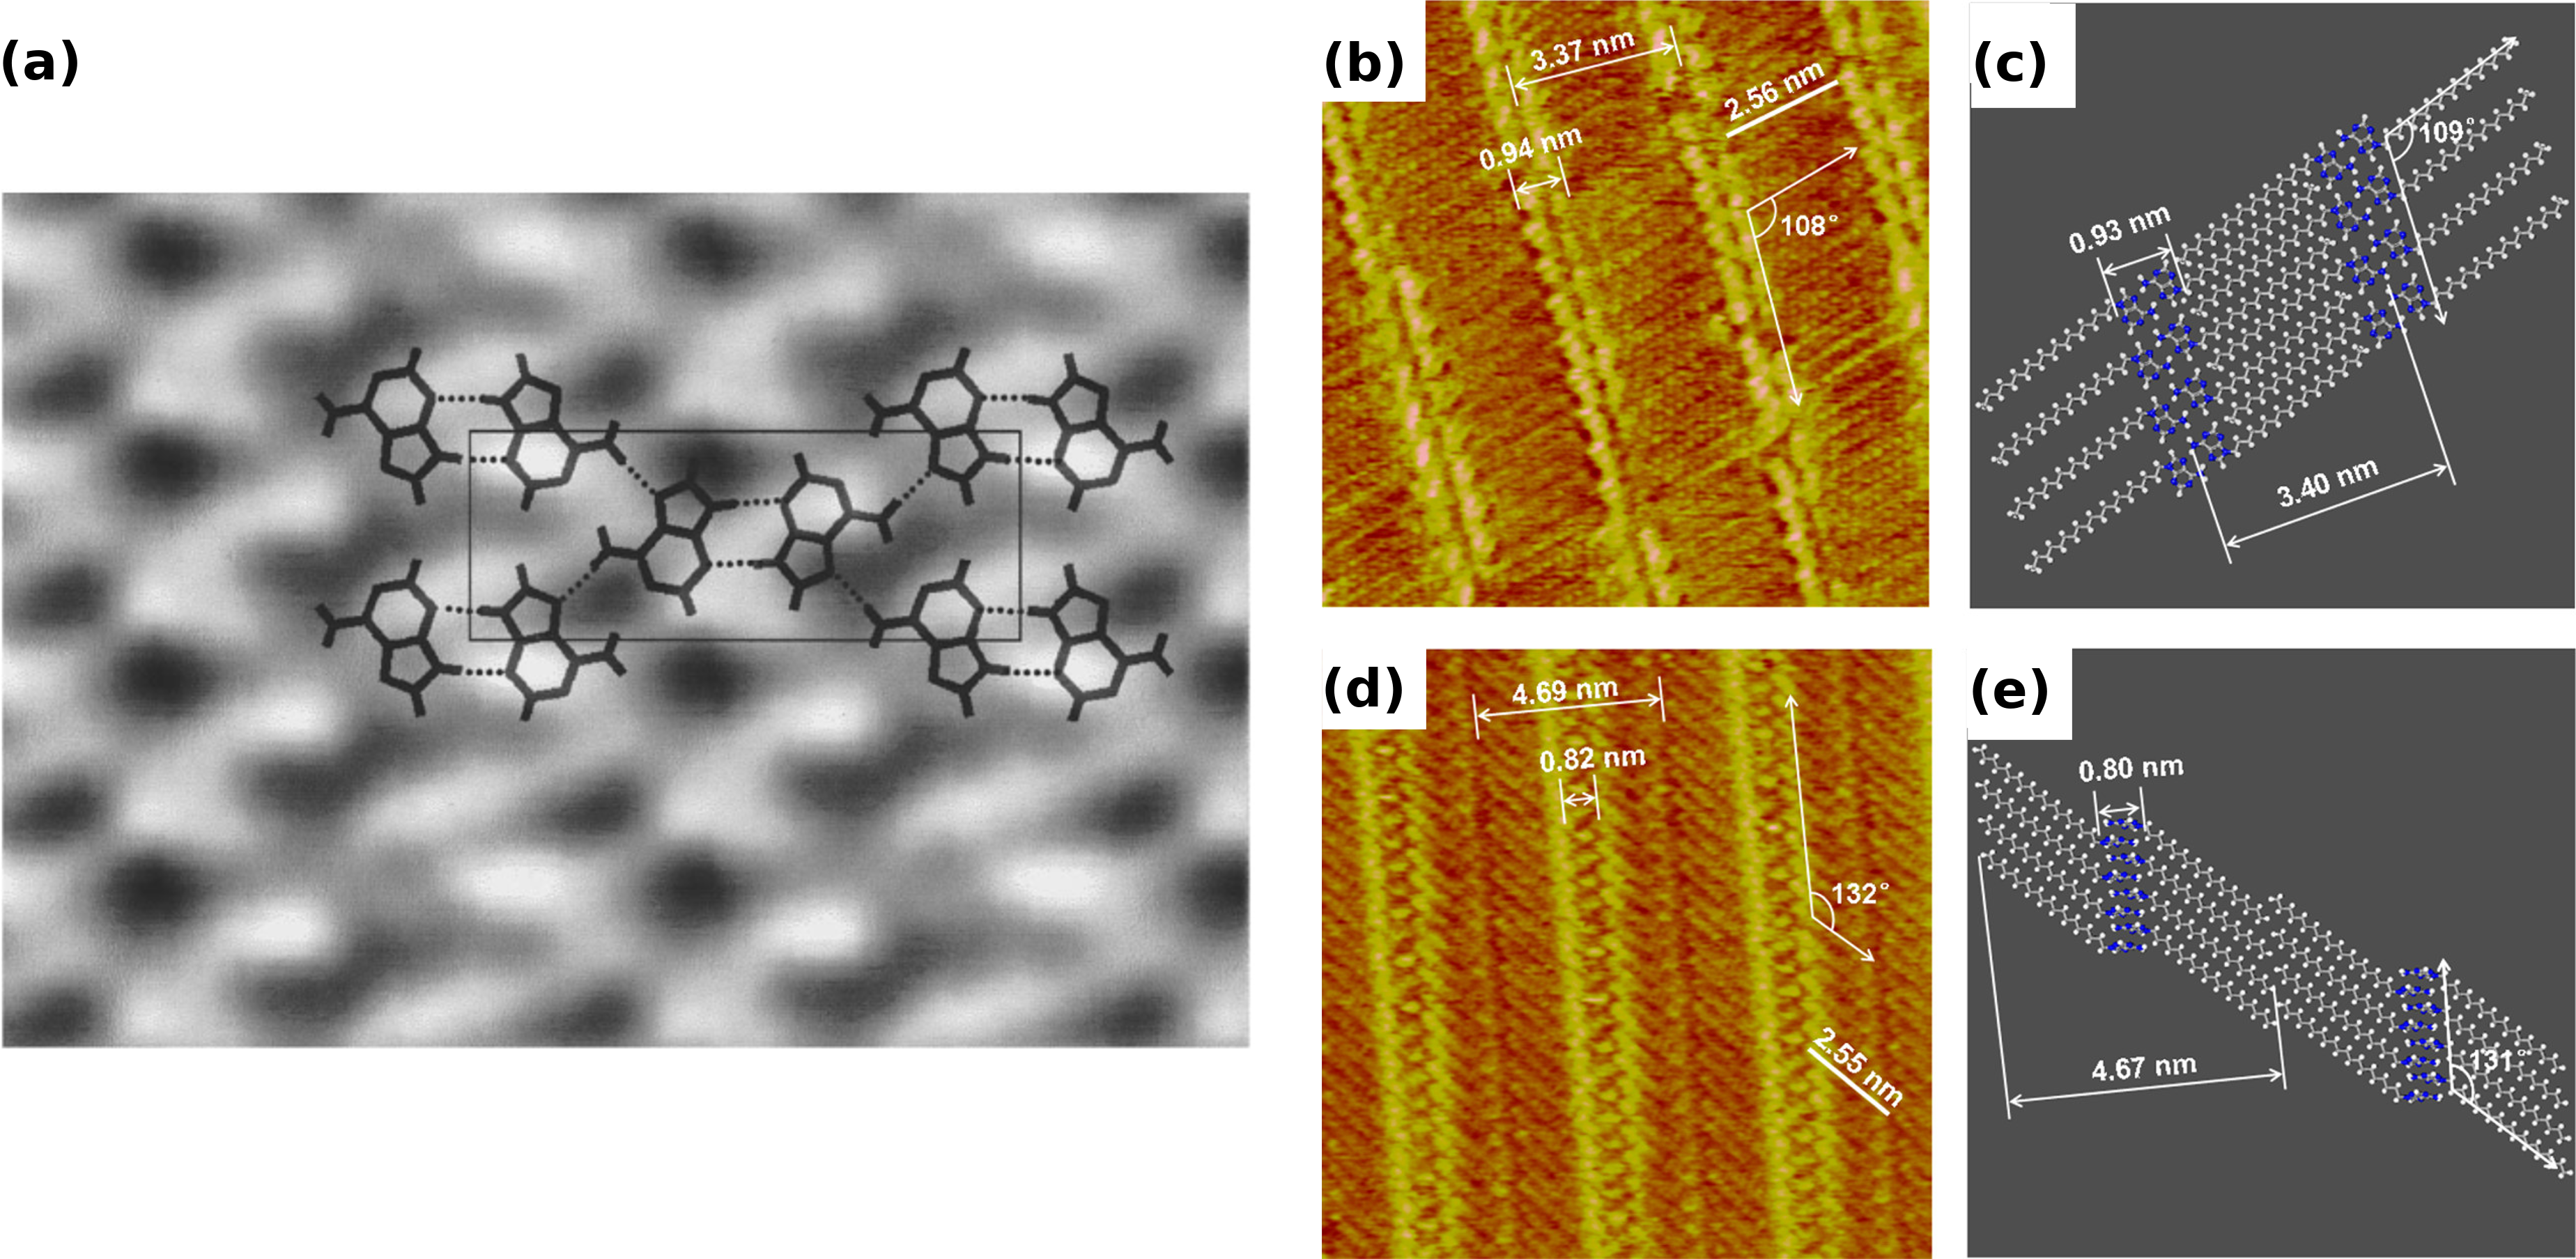
\includegraphics[width=\textwidth]{Introduction/Figures/Figure4.png}
    \caption[Representative structures for adenine self-assemblies over graphene]{(a) STM image of an epitaxially grown monolayer of adenine on graphite (001) with molecule positions indicated (size of the imaged area: 48$\angstrom$*32$\angstrom$; U = 1.0 V, I = 90 pA, constant current mode). (b) High-resolution STM constant-current image of alkyl-substituted adenine (A-C20) physisorbed onto a graphite surface from 1-phenyloctane solution (12.0 nm × 12.0 nm, V\textsubscript{bias} = 0.6 V, I\textsubscript{set} = 0.7 nA). (c) Model suggestion to characterize the packing in the STM image of panel b. (d) High-resolution STM constant-current image of A-C20 physisorbed onto a graphite surface from 1-phenyloctane solution (15.0 nm × 15.0 nm, V\textsubscript{bias} = 0.7 V, I\textsubscript{set} = 0.8 nA). (e) Model suggestion to characterize the packing in the STM image of panel d. Panel a is reprinted (figure) with permission from \supercite{freund_structure_1997}. Copyright 2023 by the American Physical Society. Panels b-e is Reprinted (adapted) with permission from ref \supercite{mu_temperature-dependent_2013}. Copyright 2023 American Chemical Society. }
    \label{fig:figure5}
\end{figure}

Chi and coworkers investigated the self-assembly of a long alkyl-chain (icosane) terminated adenine derivative on a HOPG surface as a function of temperature.\supercite{mu_temperature-dependent_2013} They employed in-situ STM imaging and ab-initio DFT calculations to characterize the self-assemblies. Two distinct forms ($\alpha$- and $\beta$-) of the self-assembly were observed depending on the temperature. Interconversion between the two forms were also investigated as a function of the temperature [Figure 1.5(b-e)]. 

\paragraph{Guanine:} Spada and coworkers investigated the formation of self-assemblies in guanosine derivatives dipersed over an HOPG surface using STM imaging\supercite{gottarelli_self-assembly_2000}. They observed that the side chains (\textit{p}-(C\textsubscript{12}H\textsubscript{25}O)C\textsubscript{6}H\textsubscript{4} and C\textsubscript{9}H\textsubscript{19}) remained flat on the graphene surface, and the self-assembled mono-layer consisted of two ribbon-like arrangements of guanine molecules interacting via hydrogen bonds.

Samor\`{i} and coworkers demonstrated the formation of self-assembled monolayers of N$^9$-substituted guanine molecules over a HOPG surface using STM imaging and ab-initio DFT calculations.\supercite{ciesielski_nanopatterning_2010} They investigated the effect of side chain length on observed self-assemblies at the HOPG - 1,2,4-trichlorobenzene interface. The authors observed the formation of distinct self-assemblies for varying side chain lengths, with the smallest alkyl chain molecule adopting a ribbon-like structure. In contrast, the larger ones progressively moved towards crystalline structures, stabilized via hydrogen bonding interactions.

\begin{figure}
    \centering
    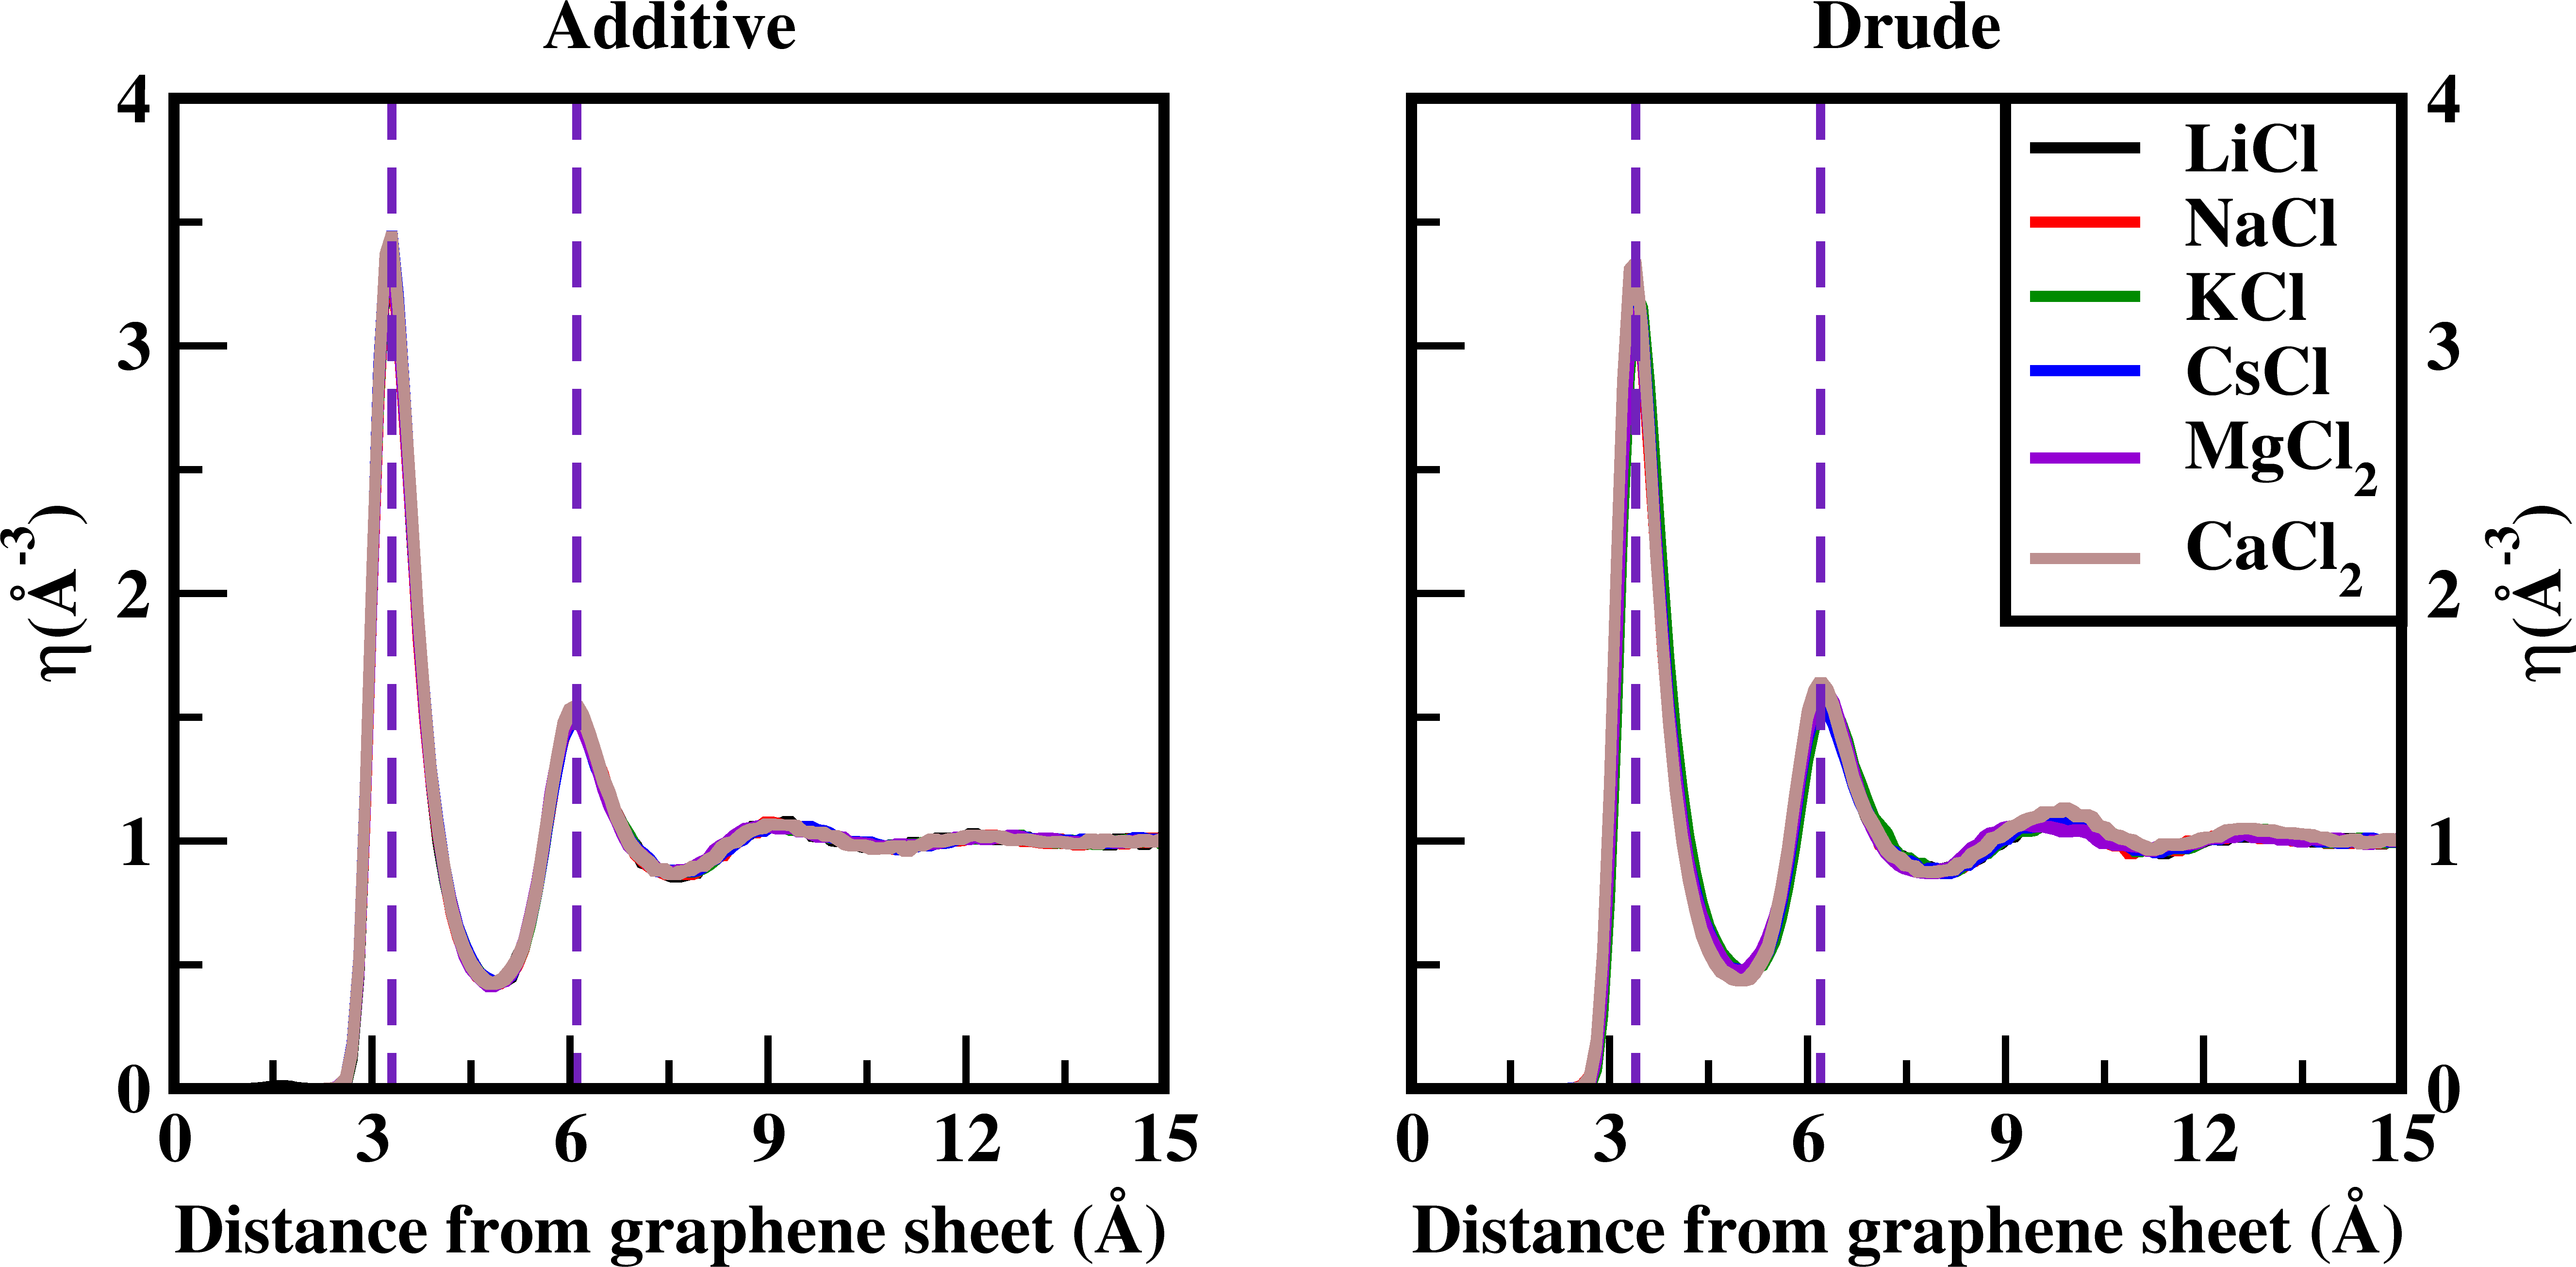
\includegraphics[width=\textwidth]{Introduction/Figures/Figure5.png}
    \caption[STM images demonstrating the structural evolution of monolayer of guanosine derivatives over graphene surface]{Consecutive STM images showing the structural evolution of a monolayer of guanosine derivatives over a 9 min time scale (time range displays in the upper right part of the images correspond to the time that was needed to reach the equilibrium after addition of reacting agents). (a), (c), and (e) show ribbon-like structure, whereas (b) and (d) exhibit G4-based architectures. Tunneling parameters: (a), (c), and (e) U$_t$=350 mV and I$_t$=15 pA; (b) and (d) U$_t$=200 mV and I$_t$=5 pA. Figure adapted (reprinted) with permission from ref. \supercite{ciesielski_dynamers_2010}. Copyright 2023 John Wiley and Sons.}
    \label{fig:figure6}
\end{figure}

Samor\`{i} and coworkers demonstrated the inter-conversion between a ribbon-like guanine supramolecular structure and G4 quartets in N$^9$-alkylguanine molecules dispersed over a graphite surface\supercite{ciesielski_dynamers_2010}. They demonstrated that the structures can be inter-converted with the addition of potassium picrate, [2.2.2]cryptand and trifluromethanesulfonic acid (HTf), where the addition of potassium ions drives the conversion towards G4 quartets, and the addition of cryptand facilitating the back-conversion to ribbon-like structures. They were able to demonstrate the successive interconversions via STM imaging, where the observed transitions in the monolayer corresponded to the two states [Figure 1.6].

Li and coworkers investigated the formation of 2D self-assembled monolayers in guanine molecules dispersed over an HOPG surface using STM imaging\supercite{xu_directional_2021}. They observed that the guanine molecules self-assembled into two distinct strcutures, one resembling a linear structure, and other corresponding to a G4 quartet. They observed that the guanine quartets are connected via intermolecular hydrogen bonds, extending the observed 2D network into a line.

We note that multiple reports of guanosine-based self-assemblies are available in the literature\supercite{spada_guanosine-based_2008,xu_directional_2021,ciesielski_dynamers_2010,ciesielski_nanopatterning_2010,gottarelli_self-assembly_2000}, and the results seem to agree that the guanine molecules tend to self-assemble into one of the three forms: either into linear chains of guanine molecules, or into G4 quartets, or into a combination of these two forms. 

\begin{figure}[h]
    \centering
    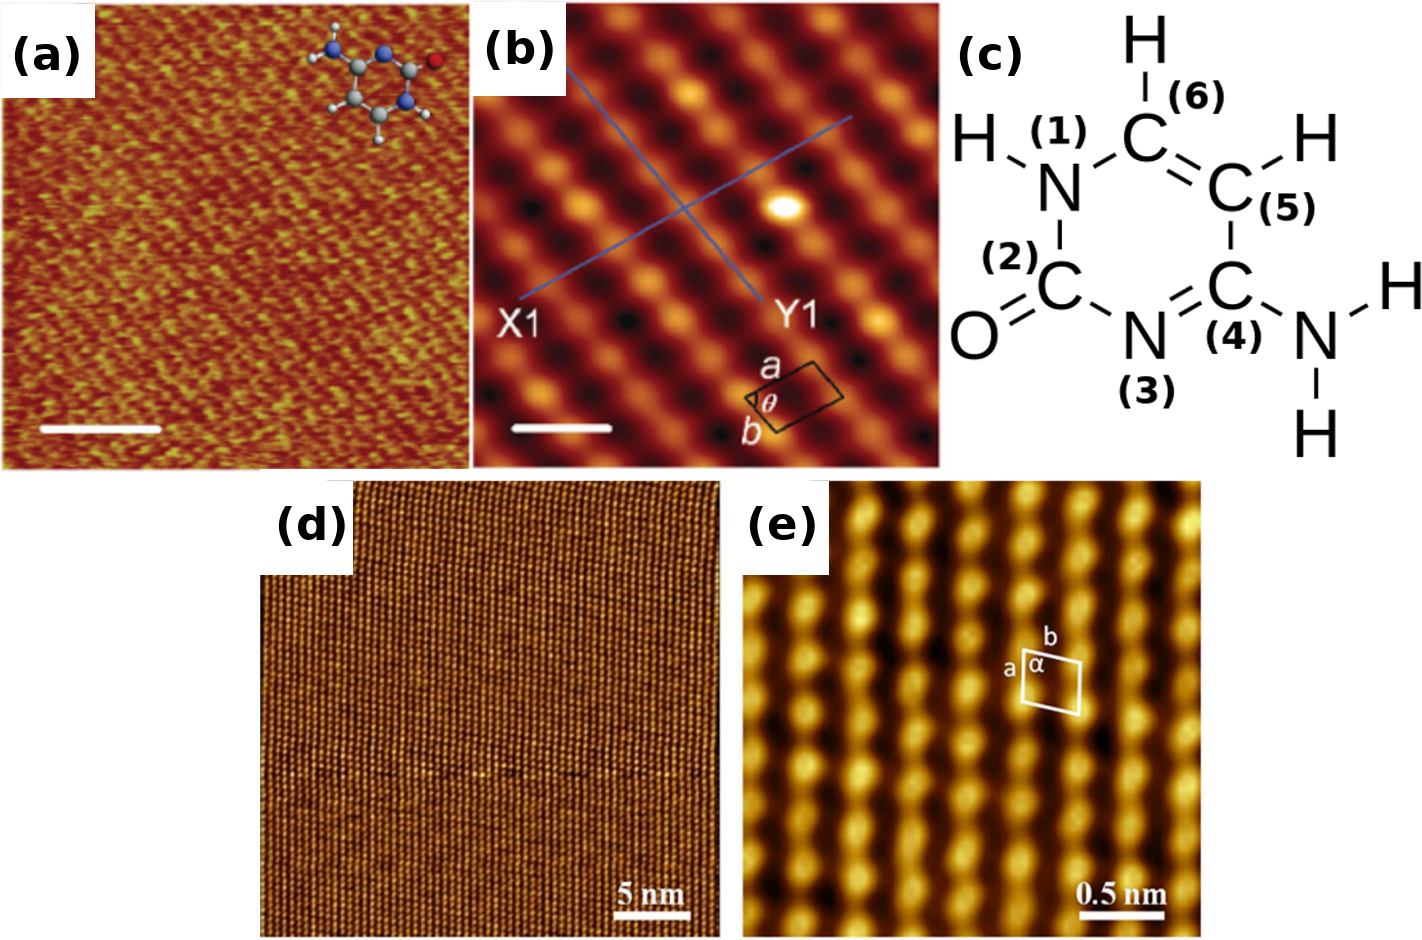
\includegraphics[width=\textwidth]{Introduction/Figures/figure_cytosine.png}
    \caption[STM images for cytosine self-assemblies over graphene]{(a) STM image of pure cytosine at water-HOPG interface (20*20  nm\textsuperscript{2};  scale bar, 5 nm; imaging tunneling current, 561.7 pA; tunneling bias, 770.3 mV). (b) Correlation-averaged zoom-in (5*5nm\textsuperscript{2}; scale bar, 1 nm). A unit cell is indicated. Reprinted (adpated) with permission from ref.\supercite{xu_coadsorption_2006}. Copyright 2023 American Chemical Society. (c) Atom numbering in cytosine molecule. (d) STM image depicting the self-assembled networks formed by cytosine molecules at the water–HOPG interface (I = 0.74nA and V = -0.42 V). High-resolution STM images show (e) self-assembled networks formed by cytosine molecules (I = 0.78nA, V = -0.45 V). Panel (d-e) adapted (reprinted) with permission from ref.\supercite{xu_directional_2021}. Copyright 2023 Elsevier.}
    \label{fig:figure7}
\end{figure}

\paragraph{Cytosine:} Besenbacher and coworkers investigated the formation of 2D self-assembled monolayers dispersed over an HOPG surface using STM imaging and DFT calculations\supercite{xu_coadsorption_2006}. They observed that cytosine molecules self-assembled in linear chains of cytosine molecules interacting via intermolecular hydrogen bonding interactions [Figure 1.7(a-b)]. From SCC-DFTB calculations, they identified that the 1D cytosine chain were formed from cytosine dimers interacting via symmetric hydrogen bonds between C2(O) and N1 atoms. We present the atom numbering used in Figure 1.7(c).

Li and coworkers also investigated the formation of 2D self-assembled monolayes in cytosine molecules disperesed over an HOPG surface using STM imaging\supercite{xu_directional_2021}. They observed the formation of an ordered 2D self-assembled structure composed of parallel 1D chains, where individual cytosine molecules form four hydrogen bonds with two neighbors, forming a chainlike structure [Figure 1.7(d-e)].

\paragraph{Thymine:} Besenbacher and coworkers investigated the formation of supramolecular self-assemblies at the interface of HOPG and 1-octanol for thymine nucleobases using STM imaging\supercite{mamdouh_supramolecular_2006}. They observed the formation of 1D chains of interacting thymine molecules, where thymine dimers self-assembled into parallel chains, which were further stabilized via inter-molecular hydrogen bonding interactions. Each thymine molecule forms four hydrogen-bonds with two of its neighbors in a chainlike structure, resulting in a zigzag arrangement of nucleobases.

\begin{figure}
    \centering
    \includegraphics[width=0.5\textwidth]{Introduction/Figures/Figure17.png}
    \caption[STM images for thymine self-assemblies over graphene]{(a) STM image depicting two adjacent domains of self-assembled monolayers of melanine and thymine nucelobases over graphite surface. (b) HR-STM image for D-I domain formed by thymine molecules. V\textsubscript{bias}=0.450 V and I\textsubscript{t}=0.102 nA. (c) Proposed model structure for thymine self-assembly. Figure adapted from ref.\supercite{zhao_investigating_2016}. Published by Springer Nature.}
    \label{fig:figure8}
\end{figure}

Liu and coworkers investigated the adsorption of thymine nucleobases at 1-octanol/HOPG interface using STM imaging.\supercite{zhao_investigating_2016} They observed the formation of a zig-zag arrangement of thymine molecules, where a thymine molecule is interacting with the neighbouring molecules via intermolecular hydrogen bonding interactions, facilitated via C2(O) and N3 atoms [Figure 1.8]. This observation is in agreement with the results from Besenbacher et al., who also investigated the formation of such self-assemblies in a very similar system.\supercite{mamdouh_supramolecular_2006}

Having discussed the experimental studies of 2D self-assemblies in canonical nucleobases disperesed over a graphene and (or) HOPG surface, we now focus on the computational investigations exploring the same phenomenon. Computational studies provide atomistic insights in processes that play an important role in the formation of the observed self-assemblies. To this end, we now summarize investigations based on all-atom molecular dynamics simulations.

\subsubsection{Computational Studies}
\paragraph{Molecular Dynamics Studies:} Heckl and coworkers investiagted the self-assembly of adenine nucelobases disperesed over a graphite surface using Dreiding II FF.\supercite{edelwirth_molecular_1998} In a previous investigation, they had observed the formation of self-assembled adenine monolayers over graphite.\supercite{freund_structure_1997} From the three dimeric assemblies which were considered to model the observed self-assembly, only one dimeric assembly was found to reach convergence after energy minimization and lattice dynamics simulations. The final assembly was observed to be composed of adenine dimers interacting via hydrogen bonding interactions [Figure 1.9].
\begin{figure}
    \centering
    \includegraphics{Introduction/Figures/Figure18.png}
    \caption[Representaive image depicting adenine self-assemblies over graphene]{2D self-assembly of adenine nucleobases over graphite surface. Hydrogen bonds are represented using dashed lines. Figure adpated with permission from ref.\supercite{edelwirth_molecular_1998}.Copyright 2023 Elsevier Science B.V.}
    \label{fig:figure9}
\end{figure}

Dutta and coworkers investigated the energetics of the formation of 2D assemblies by guanine, xanthine and hypoxanthine nucleobases over graphene, hexagonal boron nitride (\textit{h}-BN), and black phosphorene. They observed that the nucleobases retained the quartet geometry on all the investigated surfaces at lower temperatures, while significant reorganization of the nucleobases and subsequent loss of the quartet geometry were observed at higher temperatures.\supercite{mukhopadhyay_design_2018}  The authors reported a stabilizaton of $\sim$ 30 kcal/mol for the individual nucleobases involved in the quartet formation at lower temperatures, indicating the preference for the nucleobases to self-assemble into 2D assemblies. They also observed significant inter-quartet hydrogen bonding interactions between the quartets, providing extra stabilization to the 2D self-assembly.

Pandey and coworkers investigated the dynamics of guanine and cytosine nucleobases adsorbed over a graphene surface using non-polarizable additive FF MD simulations.\supercite{saikia_hierarchical_2017, saikia_dynamics_2018} They investigated the formation of self-assembled structures in guanine and cytosine nucleobases disperesed over a graphene surface in the presence and absence of solvent. They observed a significant difference in the interaction patterns observed in gaseous and aqueous phase simulations, with gaseous phase calculations predicting the formation of self-assembled structures stabilized by inter-molecular hydrogen bonding and $\pi$-stacking interactions between the nucleobases. In contrast, aqueous phase calculations predict a dispersed state with the nucleobases primarily interacting with the underlying graphene surface via $\pi$-stacking interactions [Figure 1.10(a-c)]. The loss of inter-molecular hydrogen bonding interactions between the nucleobases in the aqueous phase calculations results in a dispersed configuration. However, their observation was in starck contrast to the experimental observations\supercite{mu_temperature-dependent_2013, ciesielski_self-assembly_2013, heckl_two-dimensional_1991, freund_structure_1997} where significant hydrogen bonding interactions between the nucleobases stabilized the self-assembled monolayers.

\begin{figure}[h]
    \centering
    \includegraphics{Introduction/Figures/Figure7_cropped.png}
     \caption[Representaive image depicting guanine and cytosine self-assemblies over graphene]{(a–c) Snapshots of Gn bases (n = 6, 12, and 36) physisorbed on graphene in solvent.  Reprinted (adapted) with permission from ref \supercite{saikia_hierarchical_2017}. ACS.}
     \label{fig:figure10}
\end{figure}

% Previous studies based on ab-inito calculations have demonstrated that the strength of the non-covalent interactions between the nucleobases and the underlying graphene surface is proportional to the molecular polarizability of the nucleobases and the surface.\supercite{gowtham_physisorption_2007} Ab-inito calculations were also used in conjunction with experimental studies to explore how nucleobases self-assemble on a graphene (or graphite) surface.\supercite{xu_coadsorption_2006,ciesielski_nanopatterning_2010,wang_controlling_2014,mu_temperature-dependent_2013} However, due to the poor scaling of ab-initio methods, the applicability of these methods are limited to the study small molecular clusters or unit cells, indicating that they are not suitable to understand the dynamics of nucleobases on a graphene surface. In constrast, Molecular Dynamics simulations offer a much more accessible pathway towards understanding such dynamics. However, we note that additive FF simulations based on fixed point charges are ill-equipped to describe molecular polarizability, leading to errenous simulation outcomes.

% To understand the effect of molecular polarizability on the dynamics of nucleobases dispersed over a graphene surface, we investigated the dynamics of nucleobases dispersed over a graphene surface using Drude polarizable FF simulations.\supercite{h_polarization_2021} We demonstrated that the inclusion of polarizability plays a vital role in determining the dynamics of the nucleobases dispersed over the graphene surface. We observed the formation of ordered self-assembled structures by cytosine nucleobases adsorbed over a graphene surface, where strong inter-molecular hydrogen bonding interactions stabilized the self-assembled structures [Figure 1.10(d)]. The non-polarizable additive FF simulations did not account for this observation.

% In the same study, we also observed significant differences in the dynamics of guanine nucleobases disperesed over a graphene surface based on the FF that was employed. In non-polarizable additive FF simulations, the nucleobases were found to form small molecular clusters composed of hydrogen-bonded dimers. In contrast, Drude FF simulations predicted a 3D assembly of nucleobases tethered to the graphene surface via nucleobase - graphene $\pi$-$\pi$ interactions. We observed that the 3D assembly was stabilized via both intermoelcular hydrogen-bonding interactions and $\pi$-$\pi$ stacking interactions.

% \begin{figure}[h]
%     \centering
%     \includegraphics{Introduction/Figures/Figure8.png}
%     \caption[Representaive image depicting cytosine self-assemblies over graphene as a function of surface coverage]{(a) Time series of the center-of-mass to center-of-mass descriptor used to identify the nucleobase assemblies observed in 0.25 M simulations. Representative structures depicting the 2D network corresponding to (b) region-I, (c) region-II, and (d) region-III of the d\textsubscript{COM–COM} time series. Representative structures of nucleobase assemblies in (e) 0.50 M and (f) 0.75 M simulations. The simulation cell is indicated in yellow color and periodic images of the cell are colored green. (b–d) Nucleobases used in the center-of-mass metric are in red (3) and orange (21). All other nucleobases are colored blue. (e) and (f) Nucleobases are color-coded with respect to the distance from the graphene sheet. Nucleobases in regions (i) (d\textsubscript{Nuc–Graph} $<$ 4.5 $\angstrom$), (ii) (4.5 $\angstrom$ $<$ d\textsubscript{Nuc–Graph} $<$ 8.5 $\angstrom$), and (iii) (d\textsubscript{Nuc–Graph} $>$ 8.5 $\angstrom$) are presented in red, blue, and green, respectively. Reprinted (adapted) with permission from ref\supercite{h_capturing_2022}. Copyright 2023 American Chemical Society.}
% \end{figure}

% In a follow-up investigation, we demonstrated the transition of self-assembled monolayers from an ordered structure to a random arrangement depending on the concentration of the adsorbate (nucleobase) molecules.\supercite{h_capturing_2022} We investigated the self-assembly behaviour of cytosine nucleobases at three distinct concentrations covering the low (0.25M), medium (0.50M) and high (0.75M) concentration limits using classical Drude polarizable FF simulations. Our investigations showed that cytosine nucleobases at low concentrations can self-assemble into ordered 2D assemblies with significant lifetime, and the ordered self-assembly undergoes a steady transition towards a random arrangement of nucleobases with no perceived order with increasing concentration [Figure 1.11]. We also note that the self-assemblies we observed at 0.25M were structurally similar to the ones observed by Besenbacher and coworkers in cytosine molecules dispersed at a HOPG - 1-octanol interface via STM imaging.\supercite{xu_coadsorption_2006}

In the next section, we focus on few studies that have investigated the formation of mixed self-assemblies, where the structures are formed between two monomers of different chemical identity. It is imperative that such self-assemblies offer an important pathway towards realizing 2D networks of tunable properties, where the interactions can be tuned by intelligent choice of the interacting partners.

\subsection{Heterogeneous Systems}
\subsubsection{Experimental Studies}
\paragraph{Adenine-Thymine:}Besenbacher and coworkers investigated the formation of supramolecular self-assemblies at the interface of HOPG and 1-octanol using adenine and thymine nucleobases by employing STM imaging and DFT calculations.\supercite{mamdouh_supramolecular_2006} They observed the formation of a distinct AT supramolecular assembly which was constitutionally different from AA and TT pairings. From STM imaging, they observed two distinct regions: one row containing a cyclic substructure and another containing a 1D single chain, with the 1D chain interweaved between the rows containing cyclic substructures. They concluded from combinatorial DFT calculations that the observed AT heterostructure originates from interactions between two distinct subunits: two quartets of AT type and two sets of AA type [Figure 1.11(a-c)].

\begin{figure}
    \centering
    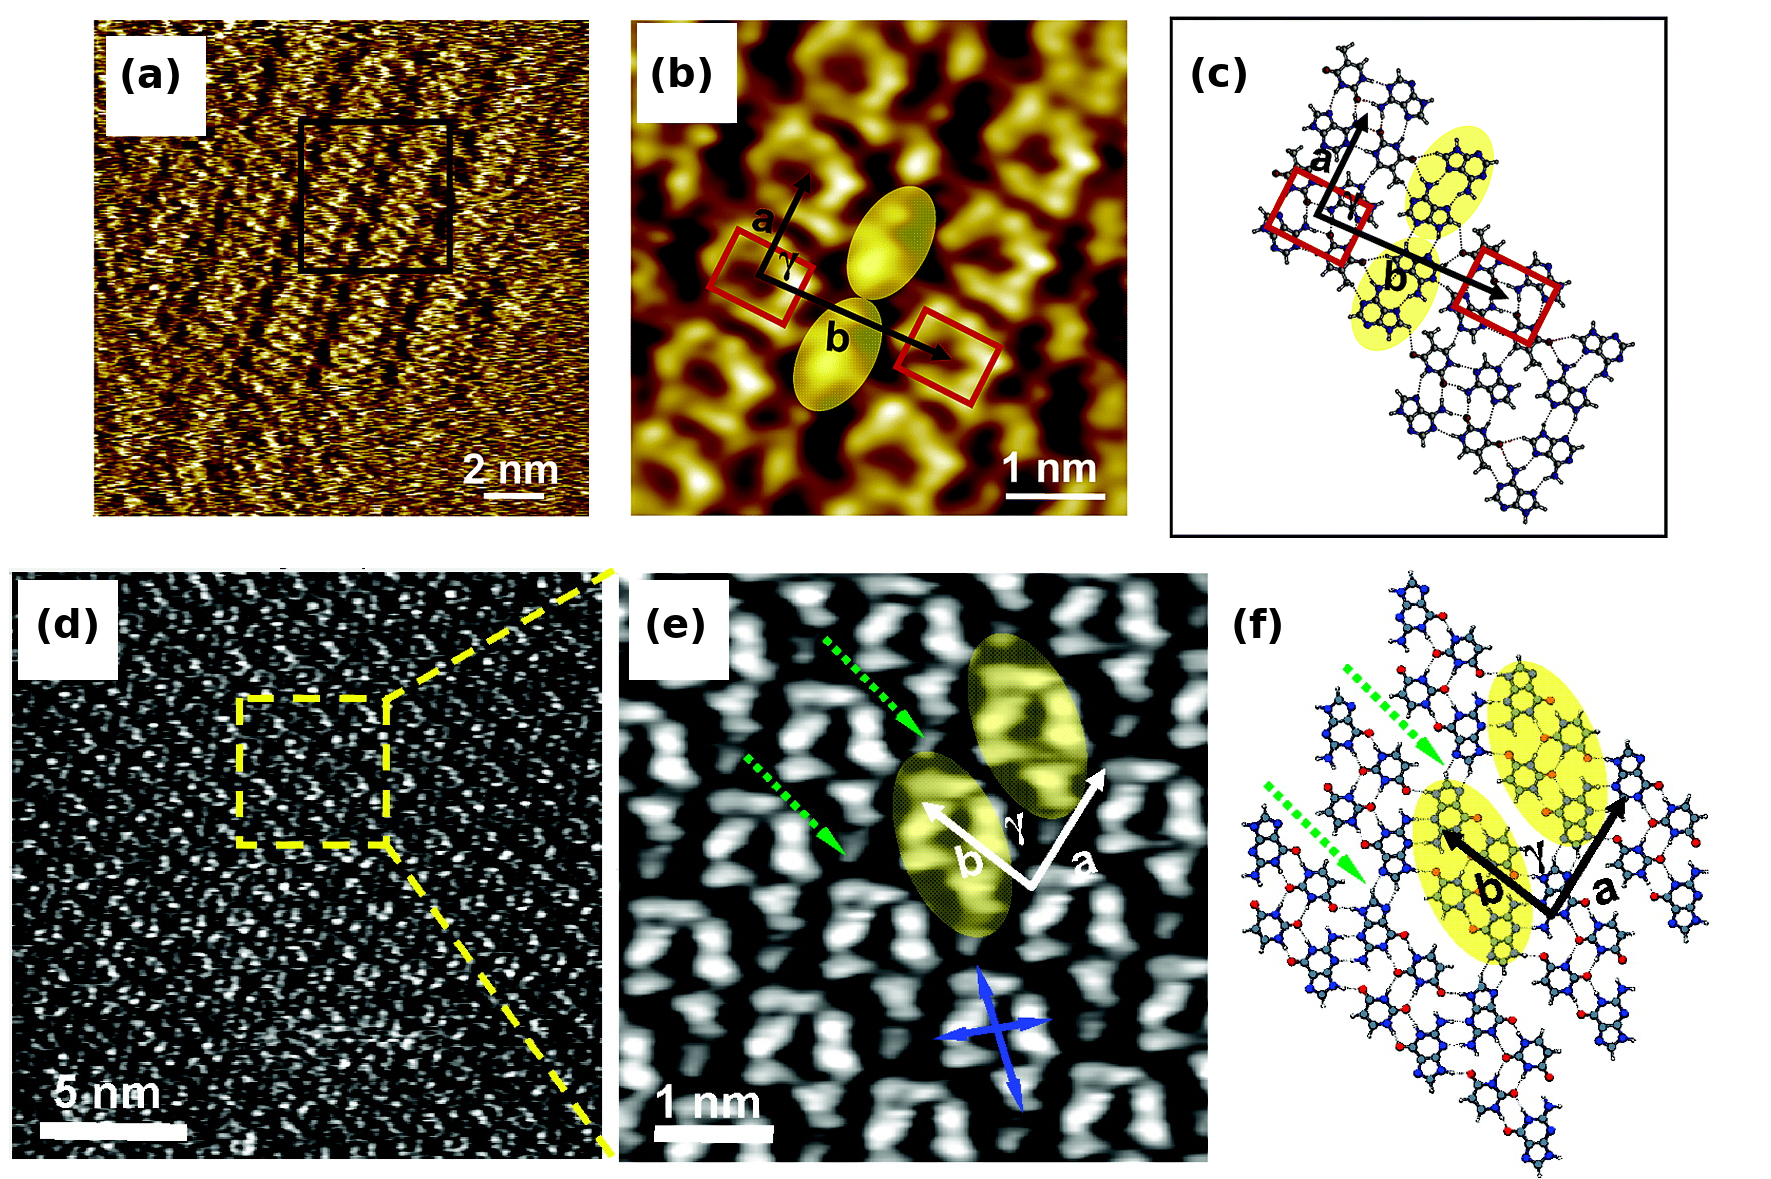
\includegraphics{Introduction/Figures/Figure10.png}
    \caption[STM images of A-T and G-U mixtures at the 1-octanol/graphite interface]{(a) STM image of A+T mixture at the 1-octanol/graphite interface. The tunneling parameters are I\textsubscript{tunn} = 1.2 nA and V\textsubscript{bias} = -447.4 mV. (b) Correlation-averaged zoom-in image of the area indicated in image (a) by a black square. (c) Calculated model suggesting that each cycle is composed of four molecules: 2A+2T, leading to reverse Hoogsteen A-T-A-T quartets adjacent to homochiral chains of A-A dimers. Cycles and A-A dimers are indicated with red rectangles and yellow ovals, respectively. The unit cell is indicated in black. Reprinted (adapted) with permission from ref \supercite{mamdouh_supramolecular_2006}. Copyright 2023 American Chemical Society. (d) High-resolution STM images of GU-base pairs at the 1-octanol/graphite interface. (e) zoom-in image of the yellow area indicated in A. Tunneling parameters are I\textsubscript{tunn} = 0.70 nA, V\textsubscript{bias} = 589.0 mV. (f) Molecular structure proposed by ab initio calculations. The GU-cyclic structures are indicated by yellow ovals, their size by blue arrows, and the unit cell lattice vectors are indicated. Green arrows indicate the hydrogen bonds between the GU-cyclic structures along unit cell vector a. Reprinted (adapted) with permission from ref \supercite{mamdouh_two-dimensional_2008}. Copyright 2023 American Chemical Society.}
    \label{fig:figure11}
\end{figure}

\paragraph{Guanine-Cytosine:} Besenbacher and coworkers investigated the formation of 2D self-assembled structures in a guanine-cytosine admixture at an HOPG-1-octanol interface using STM imaging and DFTB calculations.\supercite{xu_coadsorption_2006} They observed the formation of ordered self-assembly from the guanine-cytosine WC pairs formed from a 1D arrangement of interacting guanine and cytosine molecules. From STM images, they observed the formation of three distinct regions, where regions I and II corresponded to cytosine self-assemblies and region III corresponded to guanine-cytosine networks. DFTB calculations predicted two probable generating structures for the observed guanine-cytosine self-assembly, with two symmetric hydrogen bonds between -NH\textsubscript{2} and C2(O) extending the 1D chain. 

\paragraph{Guanine-Uracil:} Besenbacher and coworkers demonstrated the formation of a 2D self-assembled heterostructures from the interaction of guanine and uracil nucleobases at the interface of a HOPG surface and 1-octanol using STM imaging and DFT calculations.\supercite{mamdouh_two-dimensional_2008} They observed that the heterostructure formed from GU pairing substantially differed from the structures generated via the homogeneous pairing of nucleobases (GG and UU). They employed a systematic combinatorial DFT investigation to identify the unit cell corresponding to the observed GU heterostructure. They observed that only one among the multiple generated unit cells explained the obtained STM data [Figure 1.11(d-f)].

\subsubsection{Computational Studies}
\paragraph{ab-initio studies:} Cort\'{e}s-Arriagada investigated the adsorption of nucleobases and base pairs on graphene uisng PBE functional and obtained the following binding energies -14.53,  -18.68, -14.53, -14.07 and -12.45 kcal/mol for adenine, guanine, cytosine, thymine and uracil, respectively.\supercite{cortes-arriagada_phosphorene_2018} They also investigated the interaction of G-C, A-T and A-U pairs with graphene and the interaction energies of -28.13, -27.44 and -25.83 kcal/mol. The authors noted that the base pairs underwent preferential adsorption in the armchair direction of the surface.

In a follow-up study\supercite{cortes-arriagada_intermolecular_2021}, the same author investigated the binding of nucleobases and base pairs with the graphene surface using ab-inito calculations at the same level of theory as the previous study\supercite{cortes-arriagada_phosphorene_2018}. In this study, the author also investigated the effect of solvation on the binding energies using the conductor-like polarizable continuum model (CPCM) available in ORCA. The binding energies obtained for gas-phase (solvated) system were -12.91 (-10.61), -16.60 (-10.84), -12.91 (-7.61), -12.68 (-10.38), -11.07 (-8.54) kcal/mol for adenine, guanine, cytosine, thymine and uracil, respectively. They observed that the binding energies for single nucleobases interacting with a graphene surface in gas-phase followed the relative ordering of G $>$ A $>$  C $>$ T $>$ U, while the ordering became  G $>$ A $>$  T $>$ U $>$ C upon solvation. For base-pairs, the binding energies obtained were -25.14 (-20.30), -24.91 (-20.99) and -22.60 (-18.69) kcal/mol for C-G, A-T and A-U base pairs, with relative ordering being C-G $>$ A-T $>$ A-U in gas-phase and  A-T $>$ C-G $>$ A-U upon solvation. They observed that solvation drastically reduced the interaction energies between the nucleobases and the graphene surface, due to water screening the interactions between the nucleobases and the graphene surface. 

\paragraph{Molecular Dynamics Simulations:} Řezáč and coworkers investigated the differences between the propensity for hydrogen bonding interactions and $\pi$-stacking interactions between the nucleobases in three different conditions: vacuum, solvated and in the presence of solid support (graphene) using enhanced sampling MD simulations.\supercite{spiwok_free-energy_2011} They demonstrated a notable difference in the stabilizing interactions between the nucleobases in these conditions, with vacuum simulations predominantly stabilized via hydrogen-bonding interactions, while solvated systems preferred $\pi$-stacking interactions. In contrast, nucleobases preferentially interacted via hydrogen bonding interactions in the presence of solid support like graphene [Figure 1.12]. The authors reasoned that the strong preference of the nucleobases to first interact with the graphene surface via $\pi$-stacking interactions drives the later formation of the hydrogen bonding interactions between the nucleobases. This observation agrees with the calculated interaction energies: 19.1 - 26.3 kcal/mol for graphene-nucleobase $\pi$-stacking interactions, while A-T and G-C hydrogen bonds are at -13.1 and -17.5 kcal/mol, respectively.

\begin{figure}
    \centering
    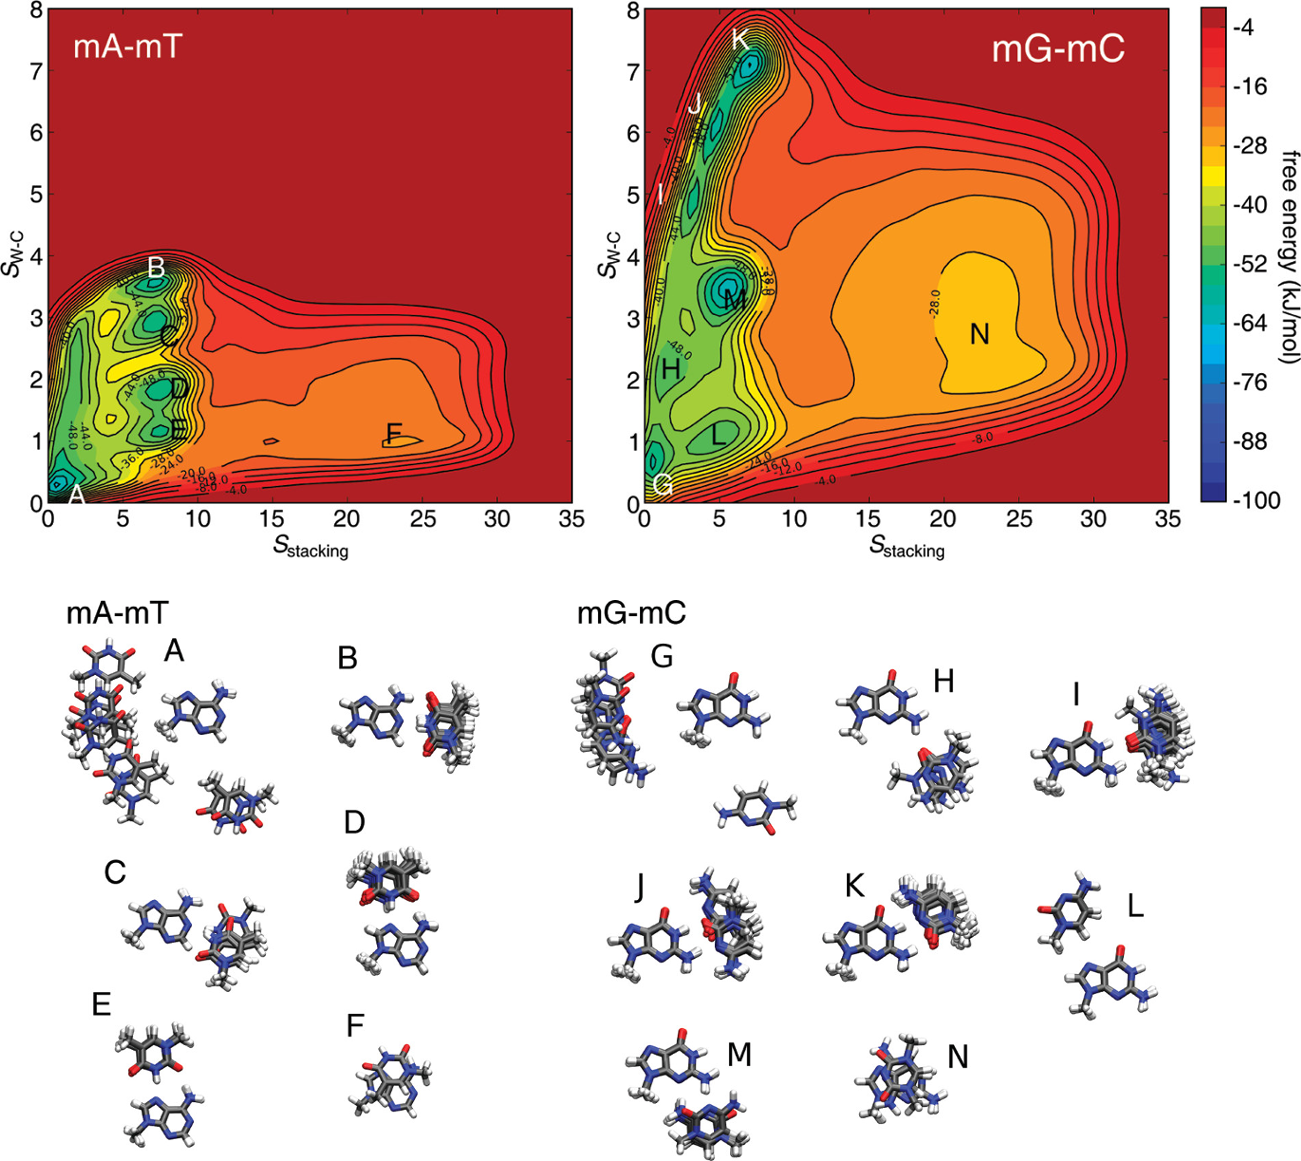
\includegraphics[width=\textwidth]{Introduction/Figures/Figure6_md.png}
    \caption[Free-energy surfaces of the association of mA–mT and mG–mC pairs on graphene. Representative structures for minima are also presented]{Free-energy surfaces of the association of mA–mT and mG–mC pairs on graphene, calculated as the negative of the metadynamics bias potential. Representative structures for Minima A–N are also presented. The axes are the collective variables describing base stacking and Watson–Crick pair formation. Snapshots of the metadynamics simulations corresponding to minima A–N. The structures of the purines are superimposed within a group. These minima are Watson–Crick pairs (B,K), stacked pairs (F,N), dissociated bases (A,G), and other hydrogen-bonded arrangements (others). Reprinted (adapted) with permission from ref \supercite{spiwok_free-energy_2011}. Copyright 2023 American Chemical Society.}
    \label{fig:figure12}
\end{figure}

Mittal and coworkers demonstrated the influence of hydrogen bonding interactions in stabilizing the DNA base pairs adsorbed over a graphite surface.\supercite{shankar_dna_2012} They employed all-atom MD simulations to investigate the binding free energies of all possible combinations of nucleoside dimer pairs interacting with the graphene surface. They observed that the formation of non-Watson-Crick-type hydrogen bonding interactions between the adsorbed nucleosides accords extra stabilization to them. They obtained a relative ordering (energies in kcal/mol) of guanine-cytosine (-3.49) $>$ adenine-guanine (-3.08) $>$ adenine-thymine (-2.82) $>$ adenine-adenine (-2.18) $>$ cytosine-thymine (-2.09) $>$ guanine-guanine (-1.92) $>$ cytosine-cytosine (-1.77) $>$ adenine-cytosine (-1.40) $>$ thymine-thymine (-1.36) $>$ guanine-thymine (-0.79) for the interacting nucleosides. The authors also note that the $\pi$-stacking interactions between the nucleobases and the graphene surface primarily drive the dynamics. This observation agrees with the results obtained by Řezáč et al.,\supercite{spiwok_free-energy_2011} who investigated the interactions between nucleobases adsorbed over a graphite surface.

Thus, we note that hydrogen bonding interactions and vdW interactions are the two major factors in the formation and stabilization of 2D self-assembled monolayer structures. An accurate description of such interactions are required to understand the mechanisms behind the formation of such structures. ab-initio calculations capture the energetics of such interactions but fail to provide insights into the time evolution of such interactions. Molecular Dynamics simulations provide insights into the time evolution of such interactions. However, non-polarizable additive simulations do not capture the formation of self-assembled structures. 

Having discussed the self-assembly of nucleobases over a graphene (graphite) surface, we now focus on the experimental and theoretical studies on the applicability of graphene nanodevices for rapid and accurate sequencing of DNA. We first describe pioneering experimental studies that demonstrated the applicability of graphene membranes as suitable candidates for DNA sequencing before discussing the potential associated issues. We then discuss the computational studies based on MD simulations to provide an atomistic insight into the translocation dynamics of the DNA strands as they move through the nanopore.

\section{Graphene Nanodevices for DNA Sequencing}
Nanopores have attracted significant attention from the scientific community as a suitable tool towards rapid and accurate detection of a wide variety of molecules.\supercite{cherf_automated_2012, manrao_reading_2012, sutherland_structure_2004, chuah_nanopore_2019, liu_two-way_2013, cai_solid-state_2021, goyal_use_2015, baaken_high-resolution_2015} The basic working principle behind nanopore sequencing is that the flow of ionic current through the nanopore is sensitive towards the translocation of the molecule through the nanopore, and the measurement of this ionic current could serve as a marker towards the identification of the specific nucleobase occupying the nanopore at that instant. One of the first demonstrations of the applicability of nanopores in the detection of ssDNA and RNA molecules came from a study by Kasianowicz and coworkers, who demonstrated that the ionic current in the system was sensitive towards the translocation of ssDNA (RNA) molecules through the $\alpha$-hemolysin pore, providing a marker to identify the translocation of molecules through the nanopore.\supercite{kasianowicz_characterization_1996} Studies based on nanopores in \textit{Mycobacterium smegmatis} porin A (MspA)\supercite{faller_structure_2004} have demonstrated that they are a suitable alternative to $\alpha$-hemolysin nanopores due to a single sensing region with a diameter of $\approx$ 1.2 nm and length of $\approx$ 0.5 nm, in contrast to the three sensing regions in $\alpha$-hemolysin with a length of $\approx$ 5 nm and a diameter of $\approx$ 1.4 nm at the smallest point\supercite{stoddart_single-nucleotide_2009,stoddart_multiple_2010}. Even though biological nanopores have been tremendously successful in sequencing applications\supercite{stoddart_single-nucleotide_2009,stoddart_multiple_2010,bates_dynamics_2003,vercoutere_discrimination_2003,nakane_nanosensor_2004,stoddart_nucleobase_2010,ayub_individual_2012,di_muccio_insights_2019,wang_retarded_2020}, they suffer from a few significant drawbacks: (i) they have high sensitivity towards temperature and pH, and (ii) they cannot be reused immediately after being used once; both of which severely restricts its operational scope.\supercite{haque_solid-state_2013}

Solid-state nanopores, such as the ones constructed in graphene and SiN\textsubscript{x}, offer a viable alternative towards biological nanopores. They have high chemical and thermal stability and can be reused multiple times, negating the drawbacks associated with biological nanopores. However, the initial excitement associated with the application of solid-state nanopores in SiN\textsubscript{x} and SiO\textsubscript{2} soon died out when it was realized that it is impossible to achieve single-molecule resolution due to the large sensing regions ($>$10 nm), leading to multiple nucleobases occupying the nanopore at the same time\supercite{li_dna_2003,storm_translocation_2005}. It was soon identified that a single-molecule resolution could be achieved by reducing the sensing area, and 2D materials such as graphene\supercite{garaj_graphene_2010,schneider_dna_2010,wells_assessing_2012,merchant_dna_2010}, \textit{h}-BN and MoS\textsubscript{2}\supercite{liu_spontaneous_2020,qiu_detection_2017,zou_spontaneous_2020,luan_spontaneous_2018} began to be investigated as suitable membranes for sequencing applications. In particular, the inter-layer spacing between two graphene layers is 3.4 $\angstrom$, which is identical to the distance between two adjacent nucleotides in a DNA strand, indicating the possibility that graphene could be a suitable membrane for DNA sequencing applications.

In this context, we now discuss pioneering experiments and simulations that demonstrated the applicability of graphene membranes for DNA sequencing applications. We divide the discussion into translocation of dsDNA and ssDNA since both these cases present different translocation behaviours.

\subsection{double-stranded DNA (dsDNA)}
\subsubsection{Experimental Studies}
\begin{figure}[!h]
    \centering
    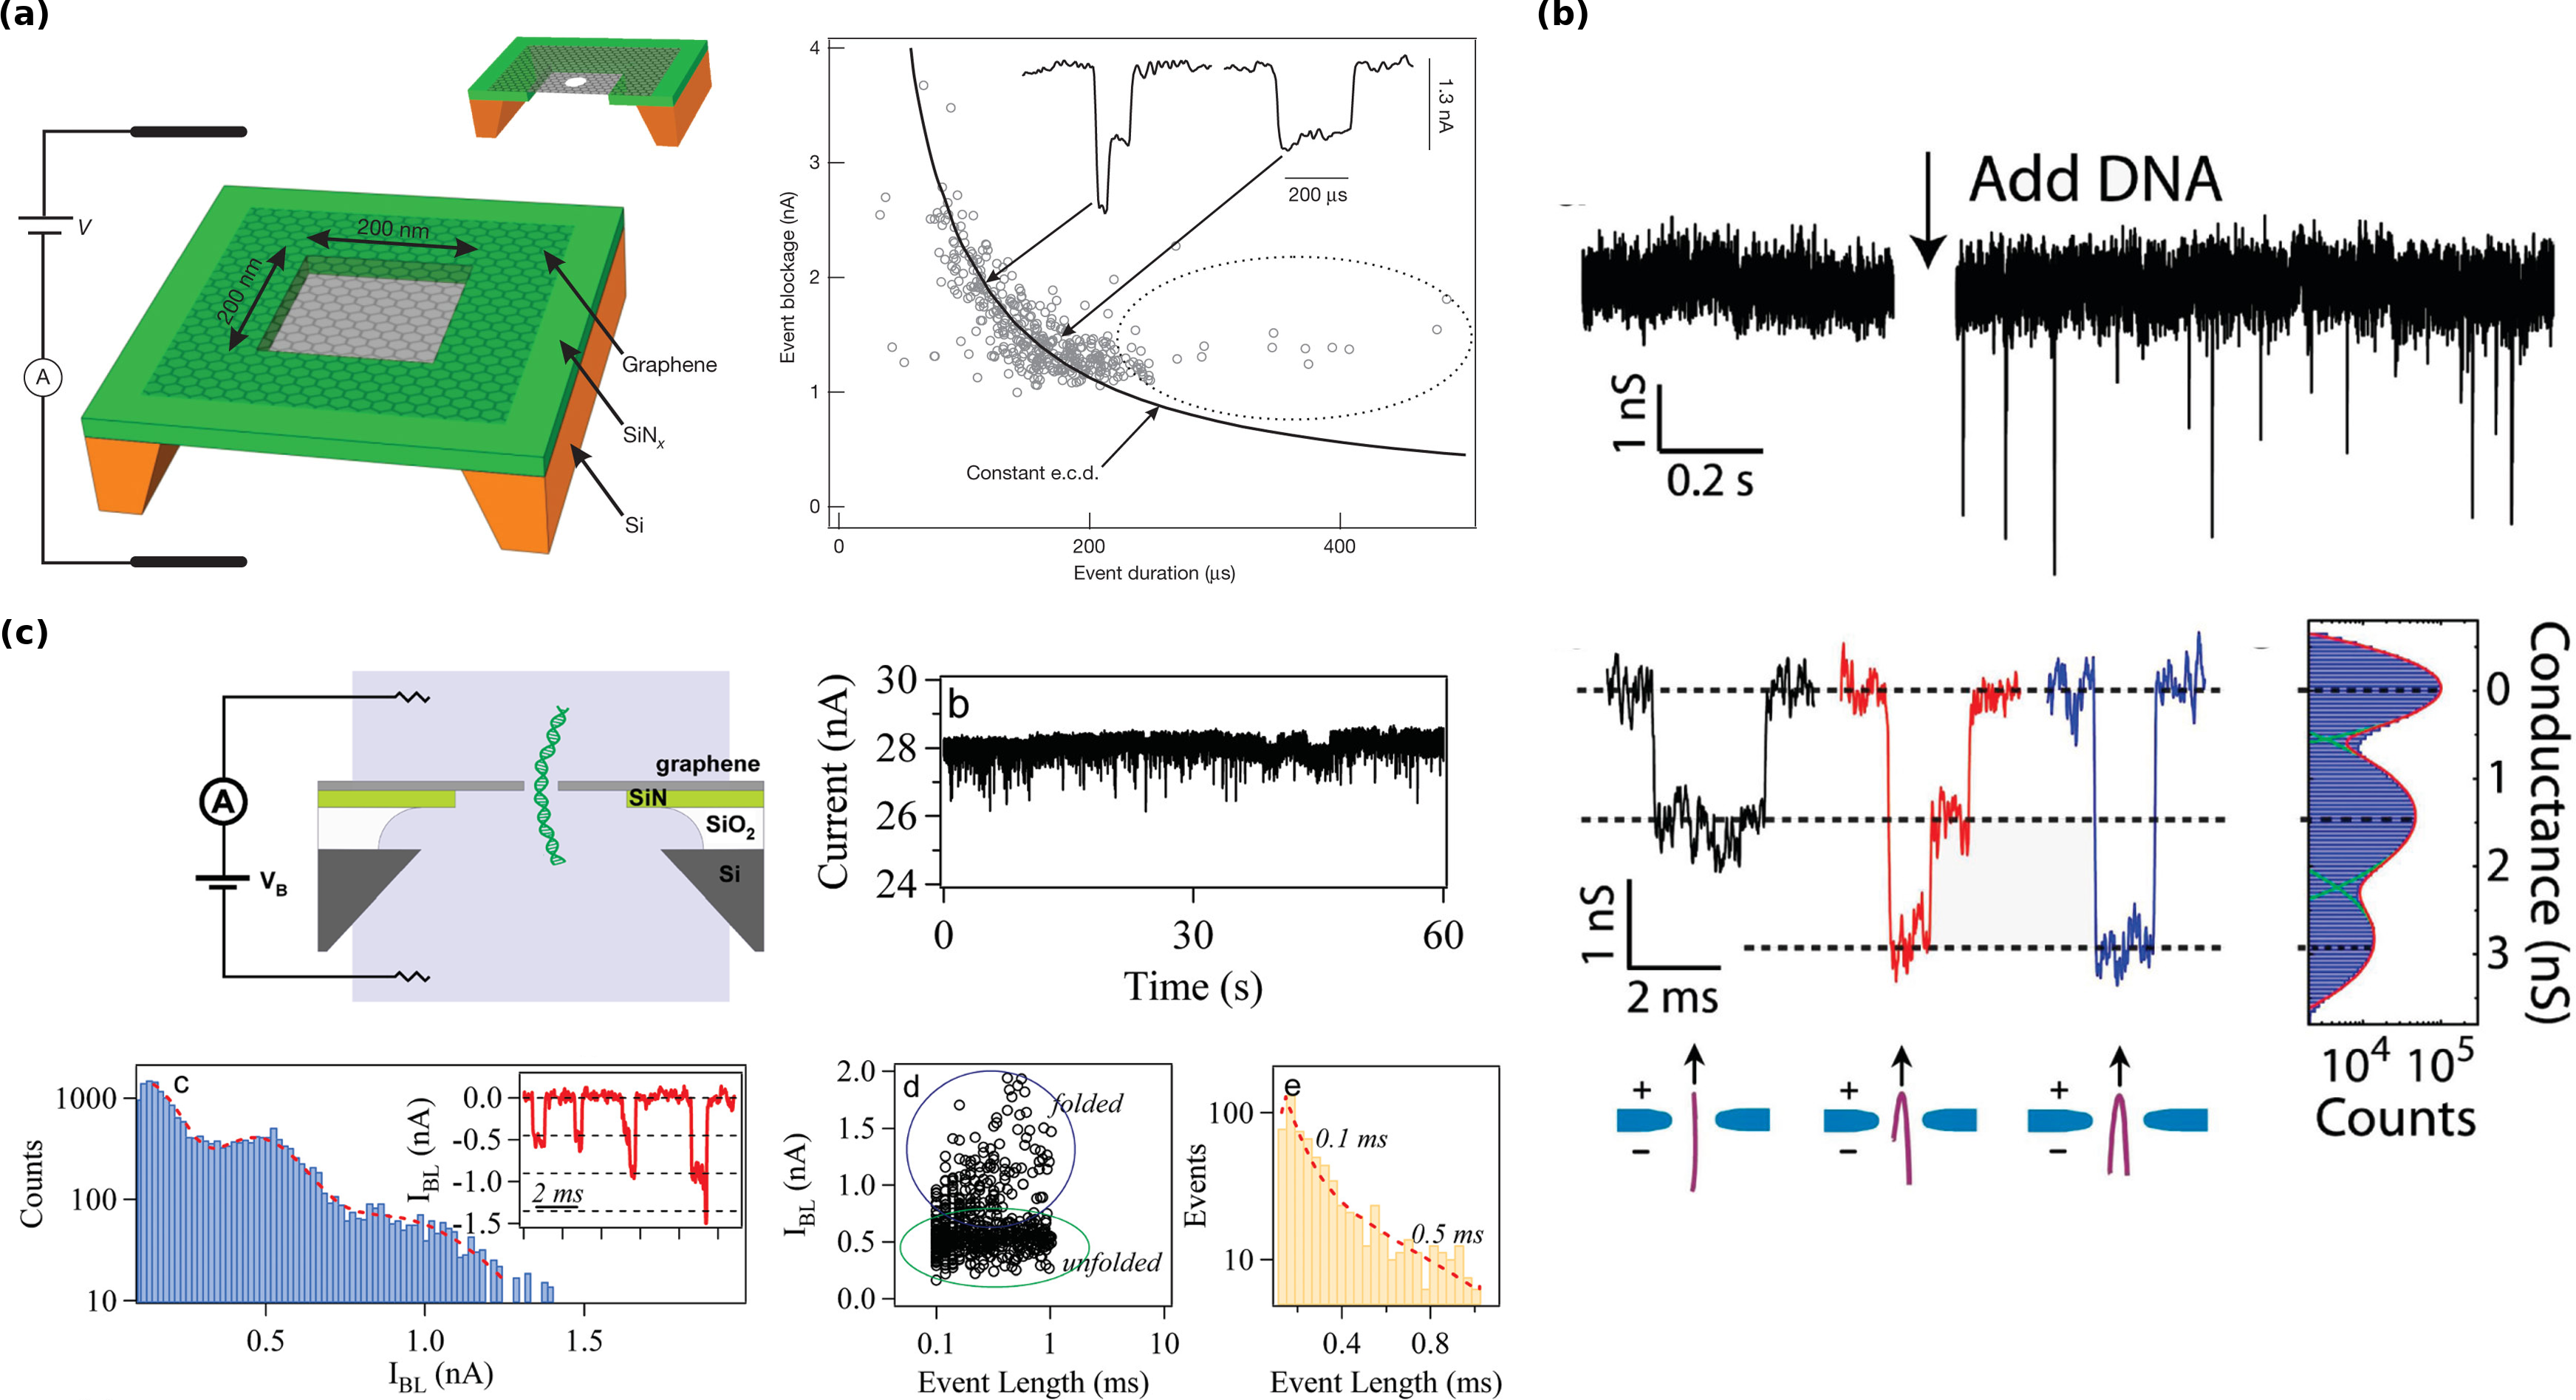
\includegraphics[width=\textwidth]{Introduction/Figures/figure_dsDNA_expt.png}
    \caption[Results from dsDNA - graphene nanopore experiments]{(a) Representaive image depicting graphene nanopore device. Ionic current trace of DNA translocation events (b) Time trace of DNA translocation events indicating unfolded, partially folded, and fully folded entries. (c) Histogram of blocked currents for measured translocation events for the nanopore device at V\textsubscript{B}=100 mV in 1 M KCl solution. Scatter plot of event length vs event depth at V\textsubscript{B}=100 mV with regions of unfolded and folded events highlighted inside the circled areas. Panel (a) reprinted (adapted) with permission from ref \supercite{garaj_graphene_2010}. Copyright 2023 Nature Publishing Group. Copyright 2023 American Chemical Society. Panel(b) reprinted (adapted) with permission from ref \supercite{schneider_dna_2010}. Copyright 2023 American Chemical Society. Panel(c) reprinted (adapted) with permission from ref \supercite{merchant_dna_2010}. Copyright 2023 American Chemical Society.}
    \label{fig:figure13}
\end{figure}

In 2010, Golovchenko and coworkers were one of the first groups to independently demonstrate that graphene membranes could be suitable for DNA sequencing.\supercite{garaj_graphene_2010} They employed an identical setup as the two other groups, with the graphene membrane placed above a SiN block and a 5-25 nm nanopore drilled into the graphene membrane by electron-beam drilling [Figure 1.13(a)]. They measured the ionic current across the graphene membrane and demonstrated the appearance of a larger blockage current associated with the translocation of DNA through the graphene nanopore.

In 2010, Dekker and coworkers independently demonstrated the applicability of graphene membranes as functional materials for DNA sequencing.\supercite{schneider_dna_2010} They demonstrated the successful translocation of a double-stranded DNA (dsDNA) through nanopores of various diameters ranging from 5-25 nm. They observed signals corresponding to three distinct modes of translocation: non-folded, partially folded and fully folded [Figure 1.13(b)]. They obtained translocation speeds of approximately 17,000 bp ms\textsuperscript{-1}, considerably slower than those achievable in SiN pores at 40,000 bp ms\textsuperscript{-1}.

Drndi\'{c} and coworkers also demonstrated one of the first experimental realizations of employing a graphene nanopore as a functional material for DNA sequencing in 2010 [Figure 1.13(c)]. They investigated a variety of devices with varied nanopore diameters (5-10 nm) and thicknesses (1-5 nm).\supercite{merchant_dna_2010} They were able to achieve higher blockage currents in comparison to traditional solid-state nanopores. They obtained an average velocity between 200,000 and 330,000 bp ms\textsuperscript{-1}, which was comparable to the velocities obtained from other solid-state nanopores. It was observed that bare graphene membranes were unsuitable for DNA sequencing applications due to the significant ion current noise and low yields, with only 10\% of the fabricated 50 devices having detectable DNA translocation. However, it was also noted that the deposition of a 5 nm thick layer of titanium dioxide resulted in a significant reduction in the noise in the observed ionic current and increased stability of the bare graphene pores.

Branton and coworkers investigated the efficacy of nanopores constructed in single-layer graphene membranes in detecting DNA bases with single-molecule resolution\supercite{garaj_molecule-hugging_2013}. The authors reported the fabrication and characterization of nanopores of varying diameters in single-layer graphene membranes and the effect of pore diameter on the detection resolution. They observed that graphene nanopores with a pore diameter comparable to the diameter of the dsDNA have high sensitivity and subnanometer resolution. The authors also employed numerical modelling to explain the experimental results and to estimate the parameters of the nanopore and the DNA molecule, such as the ion-conducting diameter, the length, and the blocking diameter. They observed that the translocation of dsDNA through the nanopore differed according to the diameter of the nanopore employed, with larger nanopores allowing for the translocation of dsDNA either in a long unfolded state or a folded state, while smaller nanopores allowed only for unfolded states. The authors also showed that dsDNA would denature at high pH, and the translocation of the ssDNA produced subsequently was considerably slower due to the interactions with the graphene surface. 

Radenovic and coworkers investigated a nanopore drilled onto a graphene nanoribbon as a suitable device for DNA detection\supercite{traversi_detecting_2013}. They investigated two markers to identify the translocation of DNA molecules through the nanopore: (i) the ionic current in the system and (ii) the transverse current flowing across the graphene nanoribbon. The authors observed that they could reliably identify the translocation events by correlating the dips (spikes) in the ionic current (transverse current) and found a significant correlation between these two events. The authors also reasoned that the random uncorrelated spikes in the ionic and transverse currents could be explained by considering that the DNA molecules can approach the nanopore without undergoing translocation, and can result in a weak blocking of the ionic current in the system. In contrast, the spikes in transverse current might have their origins in the electronic interactions between the graphene nanoribbon and charged molecules in solution.

An important issue concerning employing graphene nanopores for the reliable and efficient sequencing of dsDNA(ssDNA) is the significant 1/f noise in the experimental readouts of ionic currents. In one such study, Dekker and coworkers investigated the various factors that can lead to the observed noise in the measurements and noted that the noise was substantially reduced upon increasing the thickness of the nanopore, pointing to the mechanical fluctuations in the graphene sheet as a possible origin for the observed noise\supercite{heerema_1f_2015}. In this study, the authors investigated the following factors to determine its effect on the 1/f noise: (a) Pore diameter, (b) Salt concentration, (c) Effect of substituent groups and (d) Membrane thickness. A linear relationship was found between the pore size (diameter) and the observed noise, and a larger pore leads to a smaller noise. A very minimal correlation was observed between the salt concentration and the observed noise. It was found that the pore size and salt concentration could not explain the high 1/f noise observed in the experiments. The effect of substituent groups and the subsequent modification in the number of charge carriers on the observed noise were investigated by introducing carboxyl groups at the pore edges. No significant correlations were observed between the 1/f noise and the modulation of charge carriers, indicating that substituent groups are also not responsible for the observed noise. A significant correlation was observed between the membrane thickness (number of graphene layers) and the 1/f noise. It was found that the noise underwent significant reduction upon increasing the number of graphene layers, with a 1.5 times reduction in the noise levels when the layer thickness was increased from 1 to 20 graphene layers. The authors reasoned that the mechanical behaviour of the graphene layers was the reason for the significant 1/f noise observed in the graphene membranes. Few-layer graphene sheets can have significant oscillations in the sheets, inducing low-frequency noise in the measured ionic current readouts by modifying the ionic flux across the membrane.

In an unrelated study, Kim and coworkers also investigated the origins of 1/f noise in graphene-based devices, and they investigated devices consisting of few-layer graphene on top of quartz and silicon nitride substrates\supercite{kumar_noise_2013}. Initially, they investigated the effect of substrate on the 1/f noise in graphene. They found that the quartz-based device displayed a lower noise than the silicon nitride based device. Next, they investigated the effect of the number of layers on the noise. They observed that the few-layer graphene on a quartz device had significantly lower noise than single-layer graphene on a quartz device. They demonstrated that an FLG device would enhance the ionic current and spatial resolution and improve the signal-to-noise ratio.

\subsubsection{Molecular Dynamics Studies}
Schulten and coworkers employed all-atom MD simulations to investigate the translocation of dsDNA through a graphene nanopore, to understand its efficacy as a sequencing tool.\supercite{sathe_computational_2011} They investigated a variety of descriptors, namely - pore size, the strength of an external electric field, DNA conformation and pore charge, and its effect on the calculated ionic current. They observed that a larger pore diameter would be beneficial in capturing the DNA strand in comparison to a smaller pore, as the capture of the diffusion of the DNA strand towards the pore mouth precedes the capture of the DNA by the pore, with the non-linear potential drop across larger pores facilitating this movement. While investigating the effect of pore charge on the translocation of DNA strands, they observed that positively charged pores resulted in faster translocations than negatively charged pores due to the electrostatic repulsion between the pores and the negatively charged DNA. They also demonstrated that ionic current measurement could discern between A-T and G-C pairs. Applying a suitable external bias in MD simulations is the key to breaking A-T hydrogen bonds selectively, resulting in different ionic current signatures compared to G-C pairs [Figure 1.14(a)].

\begin{figure}
    \centering
    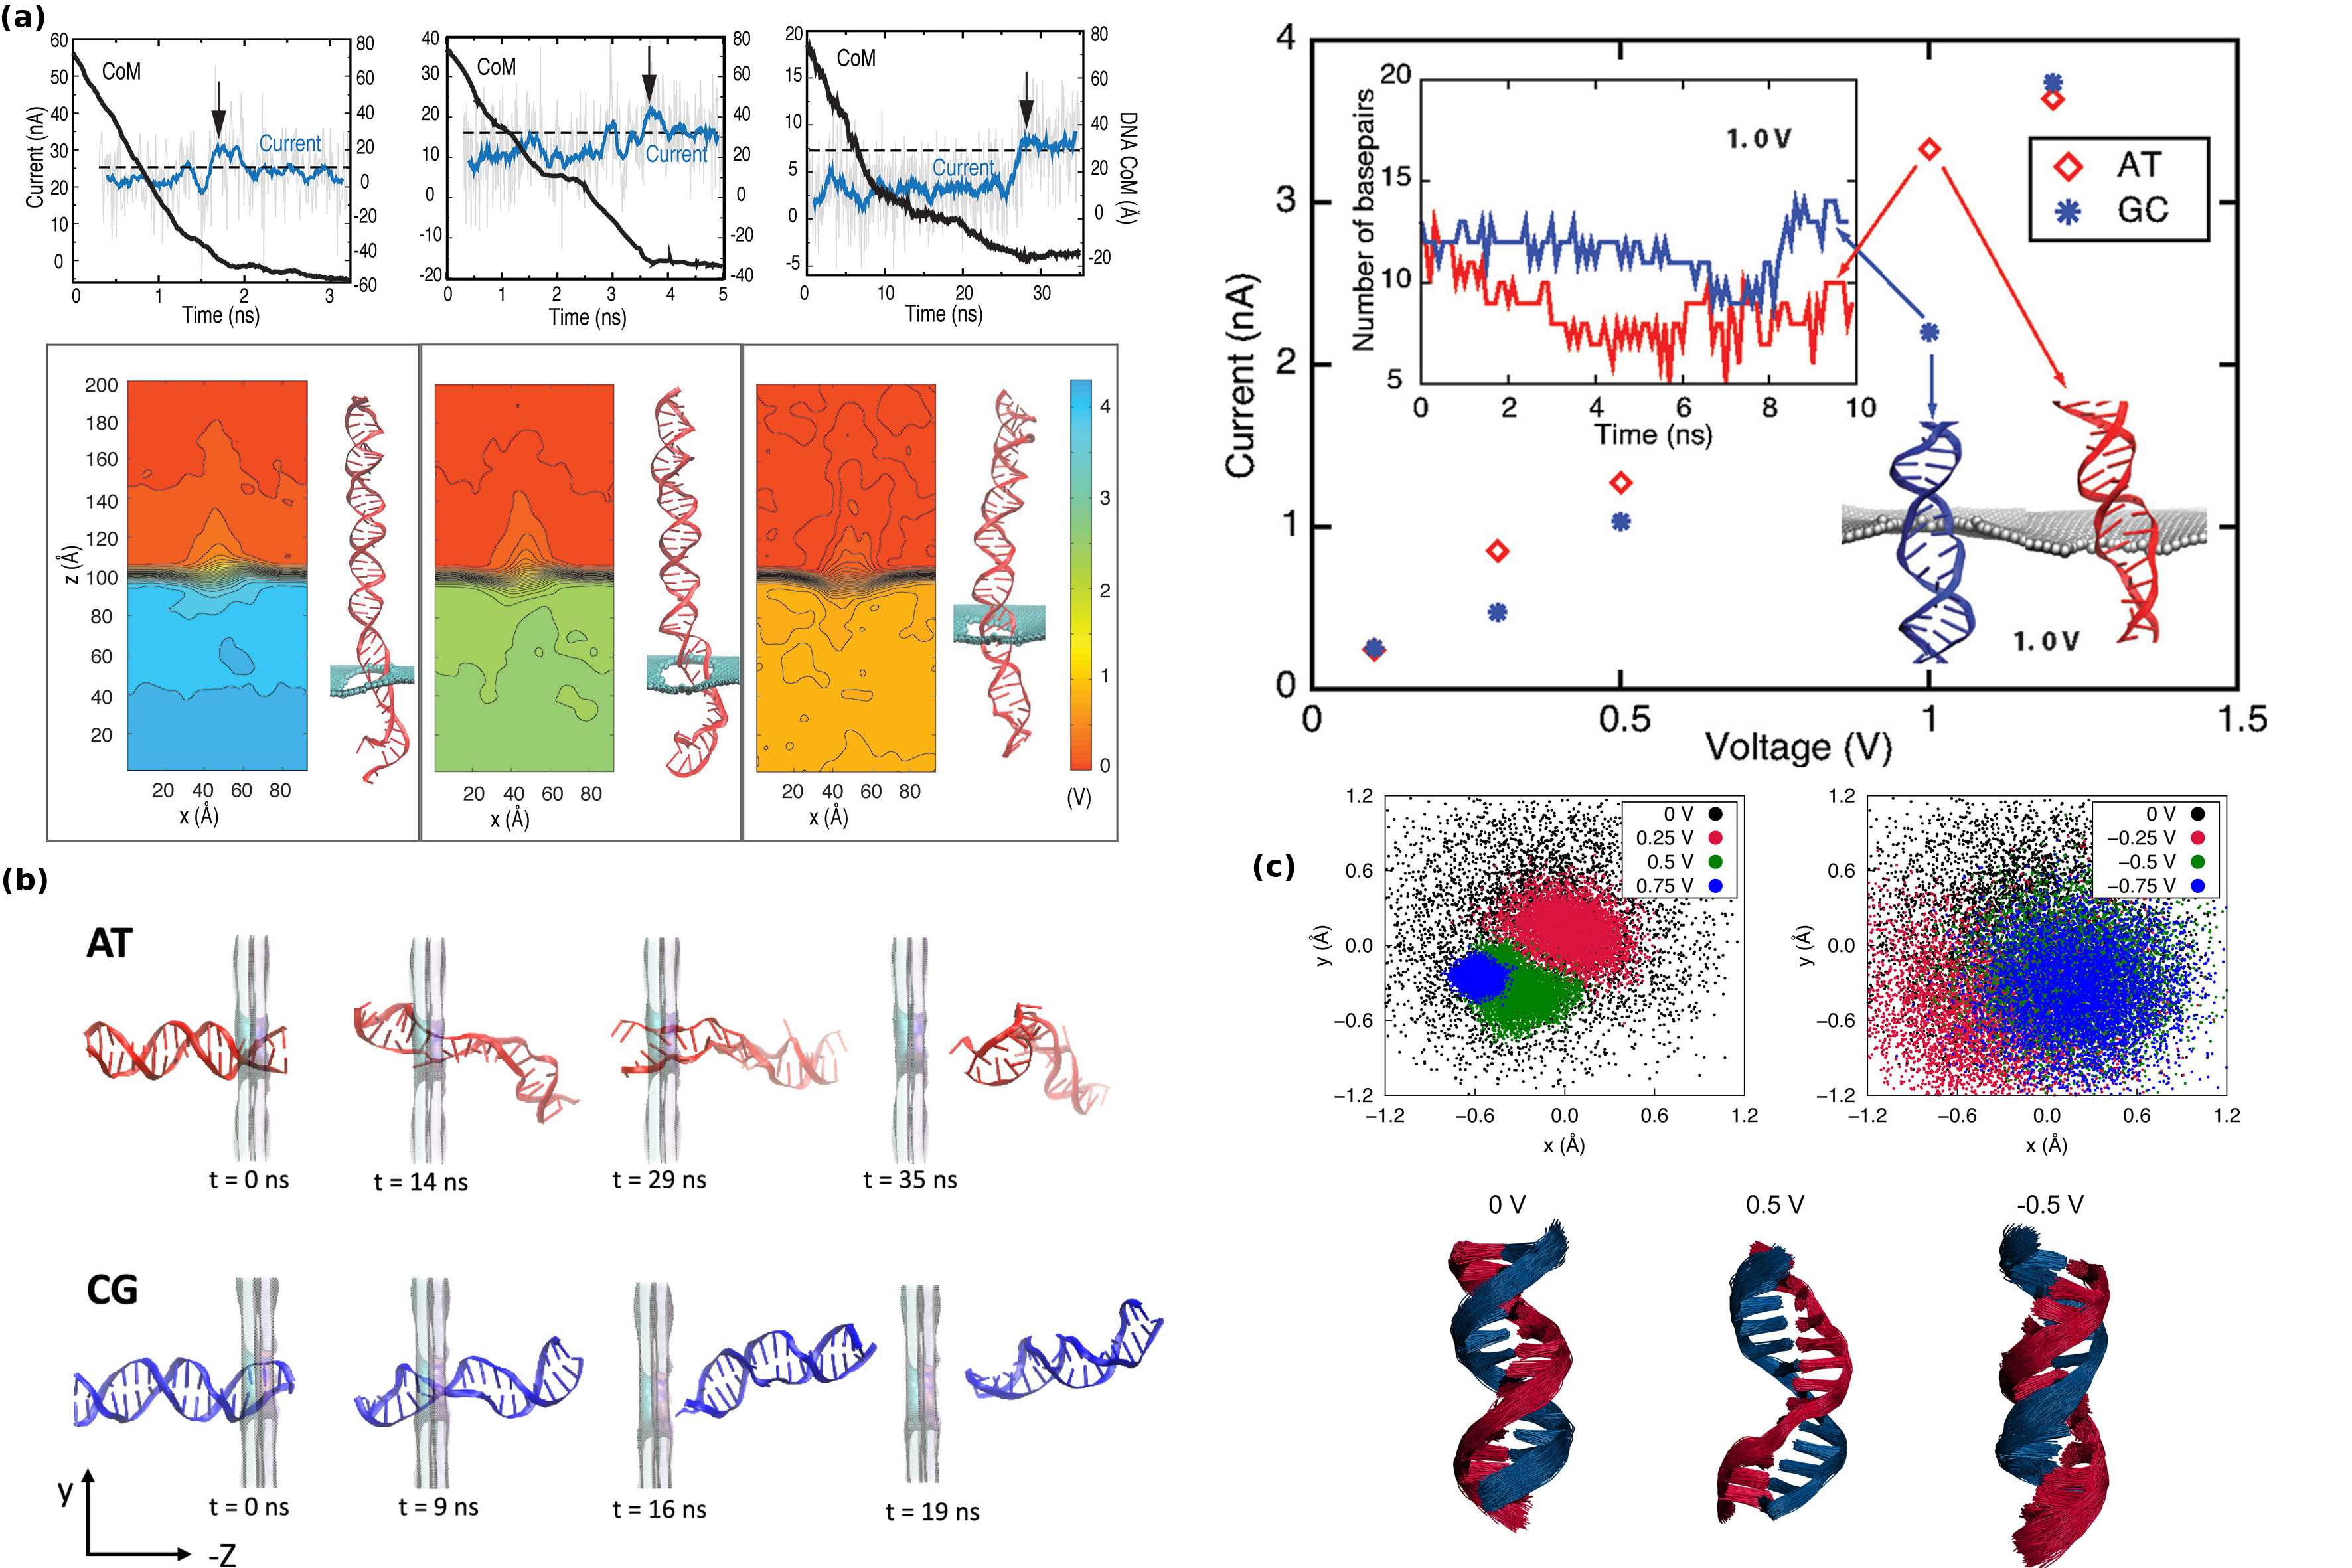
\includegraphics[width=\textwidth]{Introduction/Figures/figure_dsDNA_sim.png}
    \caption[Results from dsDNA - graphene nanopore all-atom MD simulations]{(a) Ionic current traces, CoM positions and averaged potential maps for dsDNA through graphene nanopores at various applied external biases. Ionic curent for poly-(AT)\textsubscript{20} and poly-(GC)\textsubscript{20} duplexes at different applied external biases. (b) Representative snapshots depicting the progress of dsDNA translocation through a graphene-\textit{h}-BN heterostructure nanopore. (c) Scatter diagram of CoM positions abd overlapped conformations of dsDNA at different external biases.Panel (a) reprinted (adapted) with permission from ref \supercite{sathe_computational_2011}. Copyright 2023 American Chemical Society. Panel (b) reprinted (adapted) with permission from ref \supercite{balasubramanian_dna_2021}. Copyright 2023 American Chemical Society. Panel (c) reprinted (adapted) with permission from ref \supercite{qiu_electrically_2016}. Copyright 2023 American Chemical Society.}
    \label{fig:figure14}
\end{figure}

Balasubramanian and coworkers investigated the translocation dynamics of a dsDNA through a nanopore constructed in graphene-\textit{h}-BN heterostructure using MD simulations\supercite{balasubramanian_dna_2021}. They observed that on average poly-(AT) strands required more time to complete translocations in comparison to poly-(GC) strands, with the average time being 13-24 ns for poly-(GC) strands and 28-46 ns for poly-(AT) strands. The authors reasoned that the longer translocation time of the poly(AT) sequence is based on the fact that the DNA-substrate interaction with graphene significantly distorts the double helix structure in poly-(AT) strand, leading to the dsDNA behaving as two uncorrelated ssDNA strands, and resulting in a decrease in the transverse mobility of the poly(AT) sequence (across the nanopore) consequently leading to a longer translocation time. In constrast, the double-helix structure of the poly-(GC) strand remains almost intact, leading to shorter translocation times, in general [Figure 1.14(b)].

Leburton and coworkers employed all-atom MD simulations to investigate the effect of applied external biases and the pore geometry on the conformational dynamics of the dsDNA residing within the nanopore\supercite{qiu_electrically_2016}. To this end, they first investigated the effect of multiple applied external biases on the conformational dynamics of dsDNA. They observed that a positive applied external bias reduced the fluctuations in the dsDNA due to the increased electrostatic interactions between the negatively charged dsDNA backbone and the positively charged pore walls. In contrast, they observed that a negative applied external bias resulted in more significant fluctuations in dsDNA due to the strong repulsion between the negatively charged DNA backbone and the negatively charged pore walls [Figure 1.14(c)]. To investigate the effect of pore geometry on the conformational dynamics of the dsDNA, the authors investigated the dynamics of dsDNA in a tear-drop-shaped nanopore at three voltages: -0.5 V, 0 V and 0.5 V. The authors demonstrated that at 0.5 V, the DNA strand moved towards the sharp end of the nanopore, where a slower decay of the applied external bias is expected. In contrast, the strand was located at the broader end of the nanopore during 0 V and -0.5 V simulations, indicating that fluctuations within the DNA strand can be controlled via careful choices of pore geometries and applied external biases.

Wu and coworkers investigated the effect of nanopore thickness on the translocation dynamics of a dsDNA through a graphene nanopore with varying radii and applied external biases\supercite{lv_impact_2013}. They investigated a range of nanopore thickness (1-3 layers) and pore radii (2, 2,4 and 3 nm) at applied external biases of 1-4 V, and observed that the layer thickness was inversely correlated with the speed of the translocations, with thicker nanopores slowing down the translocation of the dsDNA through the nanopore. They also observed that higher applied external biases could effect translocations even in thicker nanopores, which would otherwise be devoid of any observable translocations.

Wu and coworkers employed all-atom MD simulations to investigate the correlation between the calculated ionic current and the spatial orientations of the dsDNA strand while moving through the nanopore\supercite{lv_spatial_2014}. The authors investigated multiple systems with two different applied external biases to evaluate the effect of spatial orientations of dsDNA on the calculated ionic current. They observed that the local conformations adopted by the DNA strand significantly affected the ionic current. From further analysis of the ionic current trace and the dynamics of the dsDNA strand, they also concluded that the interactions between the DNA strand and the graphene sheet can influence the ionic current. Further, they also observed that the ionic current depends on the location of the DNA strand with respect to the nanopore.

\subsection{single-stranded DNA (ssDNA)}
\subsubsection{Experimental Studies}
\begin{figure}
    \centering
    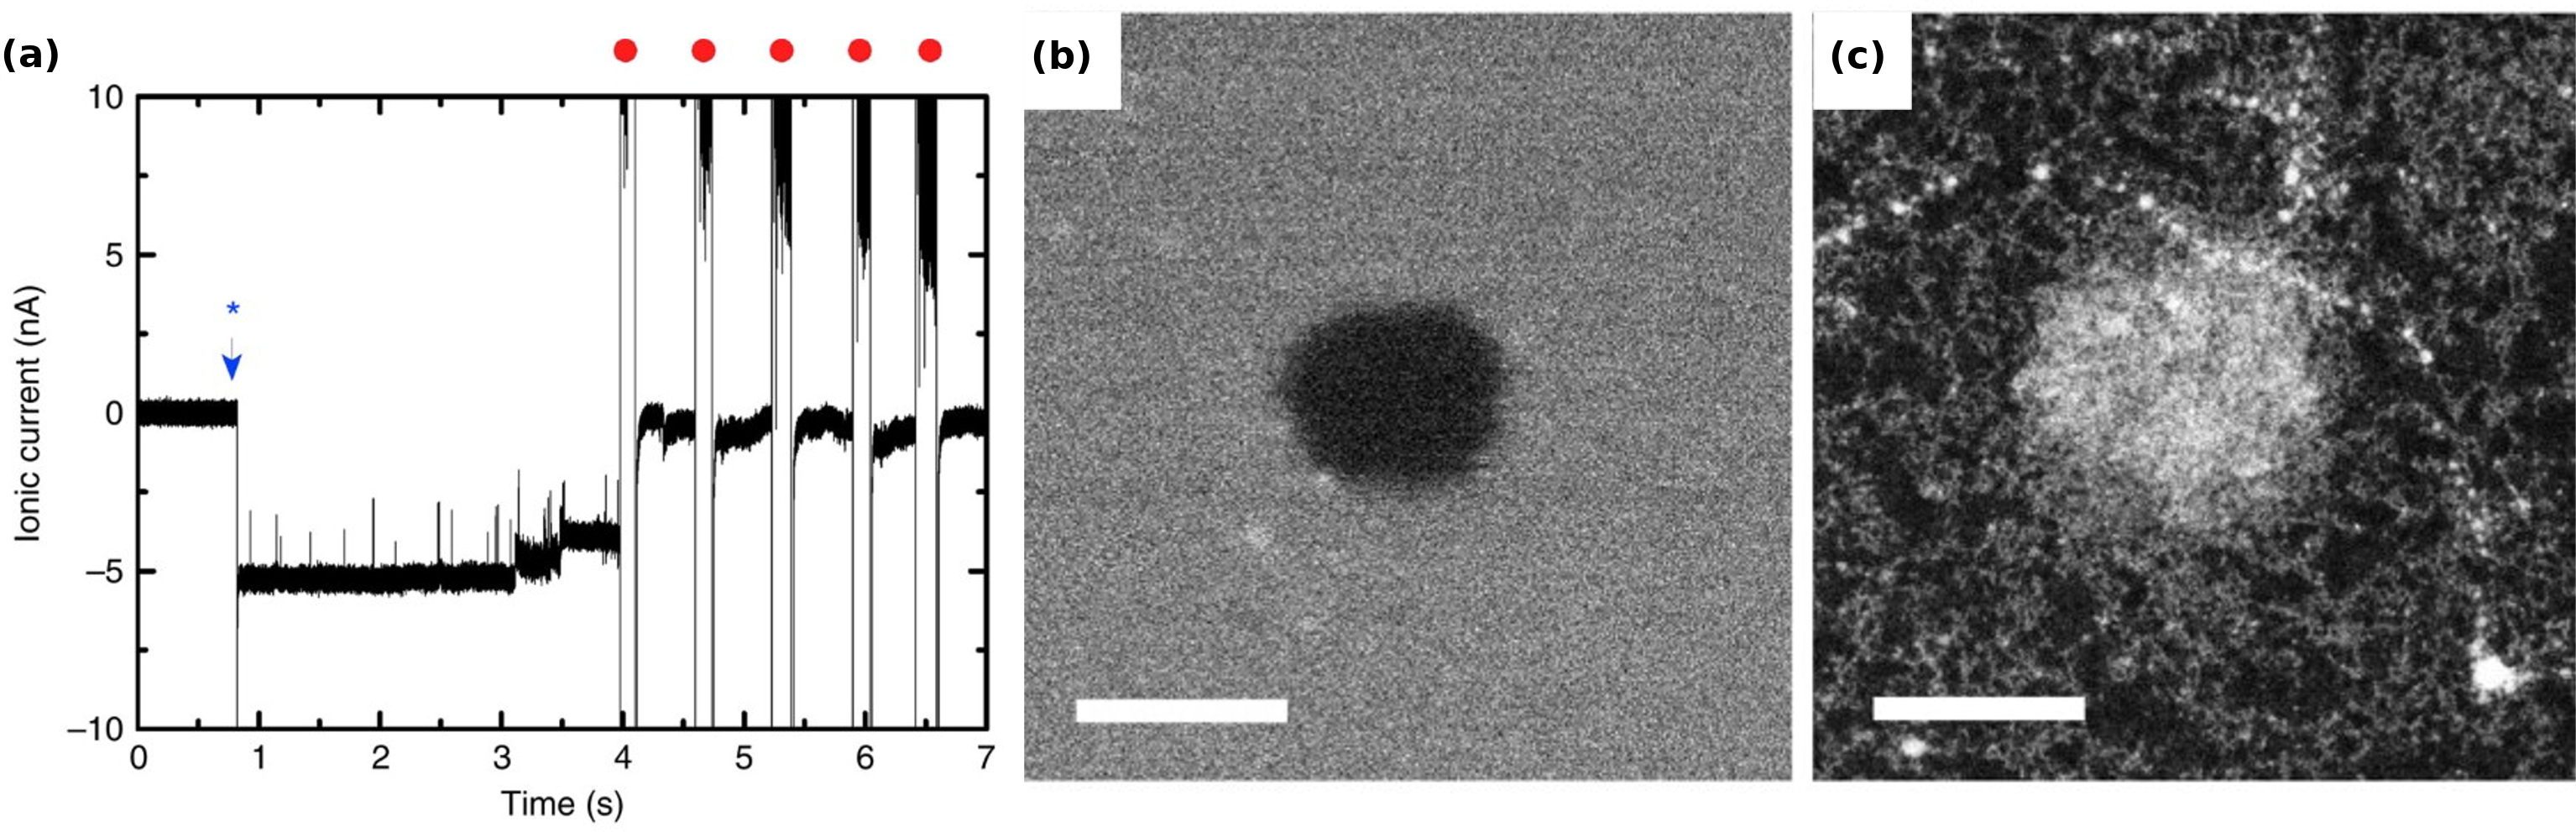
\includegraphics[width=\textwidth]{Introduction/Figures/figure_ssDNA_expt.png}
    \caption[Results from ssDNA - graphene nanopore experiments]{(a) Ionic current trace obtained for pristine graphene nanopore incubated with ssDNA. Timesteps where large 1V pulses (red dots) were applied are also indicated. (b) STM image for the pristine graphene nanopore. (c) STM image for the same nanopore after the experiment, demonstrating pore clogging. Reprinted (adapted) with permission from ref \supercite{schneider_tailoring_2013}. Copyright 2023 Nature Publishing Group.}
    \label{fig:figure15}
\end{figure}

Hydrophobic interactions between the ssDNA strand and the graphene surface are a limiting factor in the translocation of the ssDNA strand through the graphene nanopore, with significant pore clogging observed when pristine graphene membranes are employed [Figure 1.15]. Schnider and coworkers demonstrated that a SAM with a long hydrophilic alkyl chain could be a suitable anti-fouling agent to tune the interactions between the ssDNA strand and the graphene surface.\supercite{schneider_tailoring_2013} They constructed the SAM from two molecular cores - a hydrophobic aminopyrene and a tetraethyleneglycol monomethyl ether N-hydroxysuccinimide ester, where the aminopyrene molecules interact with the graphene surface and the long alkyl chain protruding out into the solution, rendering the graphene surface hydrophilic. From AFM studies, they observed that the ssDNA did not adsorb onto the SAM-coated graphene surface, even at high loading limits of 10 ng $\mu$l\textsuperscript{-1}. They also demonstrated unhindered translocations of ssDNA through the graphene nanopore, in contrast to the pristine graphene nanopore, where significant pore clogging necessitated the application of high voltage (1V) to effect translocations.

While hydrophobic interactions between the graphene surface and DNA leads to pore clogging, slowing down the transport of DNA across the graphene membrane is also essential to achieve sufficient temporal resolution in ionic current measurements. To this end, Aksimenteiv and coworkers constructed two devices - a graphene-alumina-graphene membrane and an alumina-graphene-alumina membrane to investigate the translocation dynamics.\supercite{banerjee_slowing_2015} They investigated the transport of dsDNA and ssDNA through these membranes. For ssDNA translocation, they observed a significant reduction in the translocation velocity ($\approx$ 180 nt ms\textsuperscript{-1}) compared to a native alumina membrane ($\approx$ 550 nt ms\textsuperscript{-1}) due to the increased interaction between the ssDNA and graphene surface. The hydrophobic interactions between the nucleobases and the graphene surface are absent for dsDNA for two reasons: (a) because of  Watson-Crick hydrogen bonding interactions and (b) the presence of a negatively charged phosphate backbone. Thus, they underwent translocations significantly faster compared to ssDNA, with a translocation velocity of 2500 bp ms\textsuperscript{-1}, which is approximately an order of magnitude faster than the translocation velocity for an ssDNA through a graphene-alumina-graphene membrane. The difference in translocation speeds for ssDNA and dsDNA demonstrated that the hydrophobic interactions between the graphene surface and the ssDNA could result in longer dwell times and significantly better temporal resolution in ionic current measurements.

\subsubsection{Molecular Dynamics Studies}
\begin{figure}
    \centering
    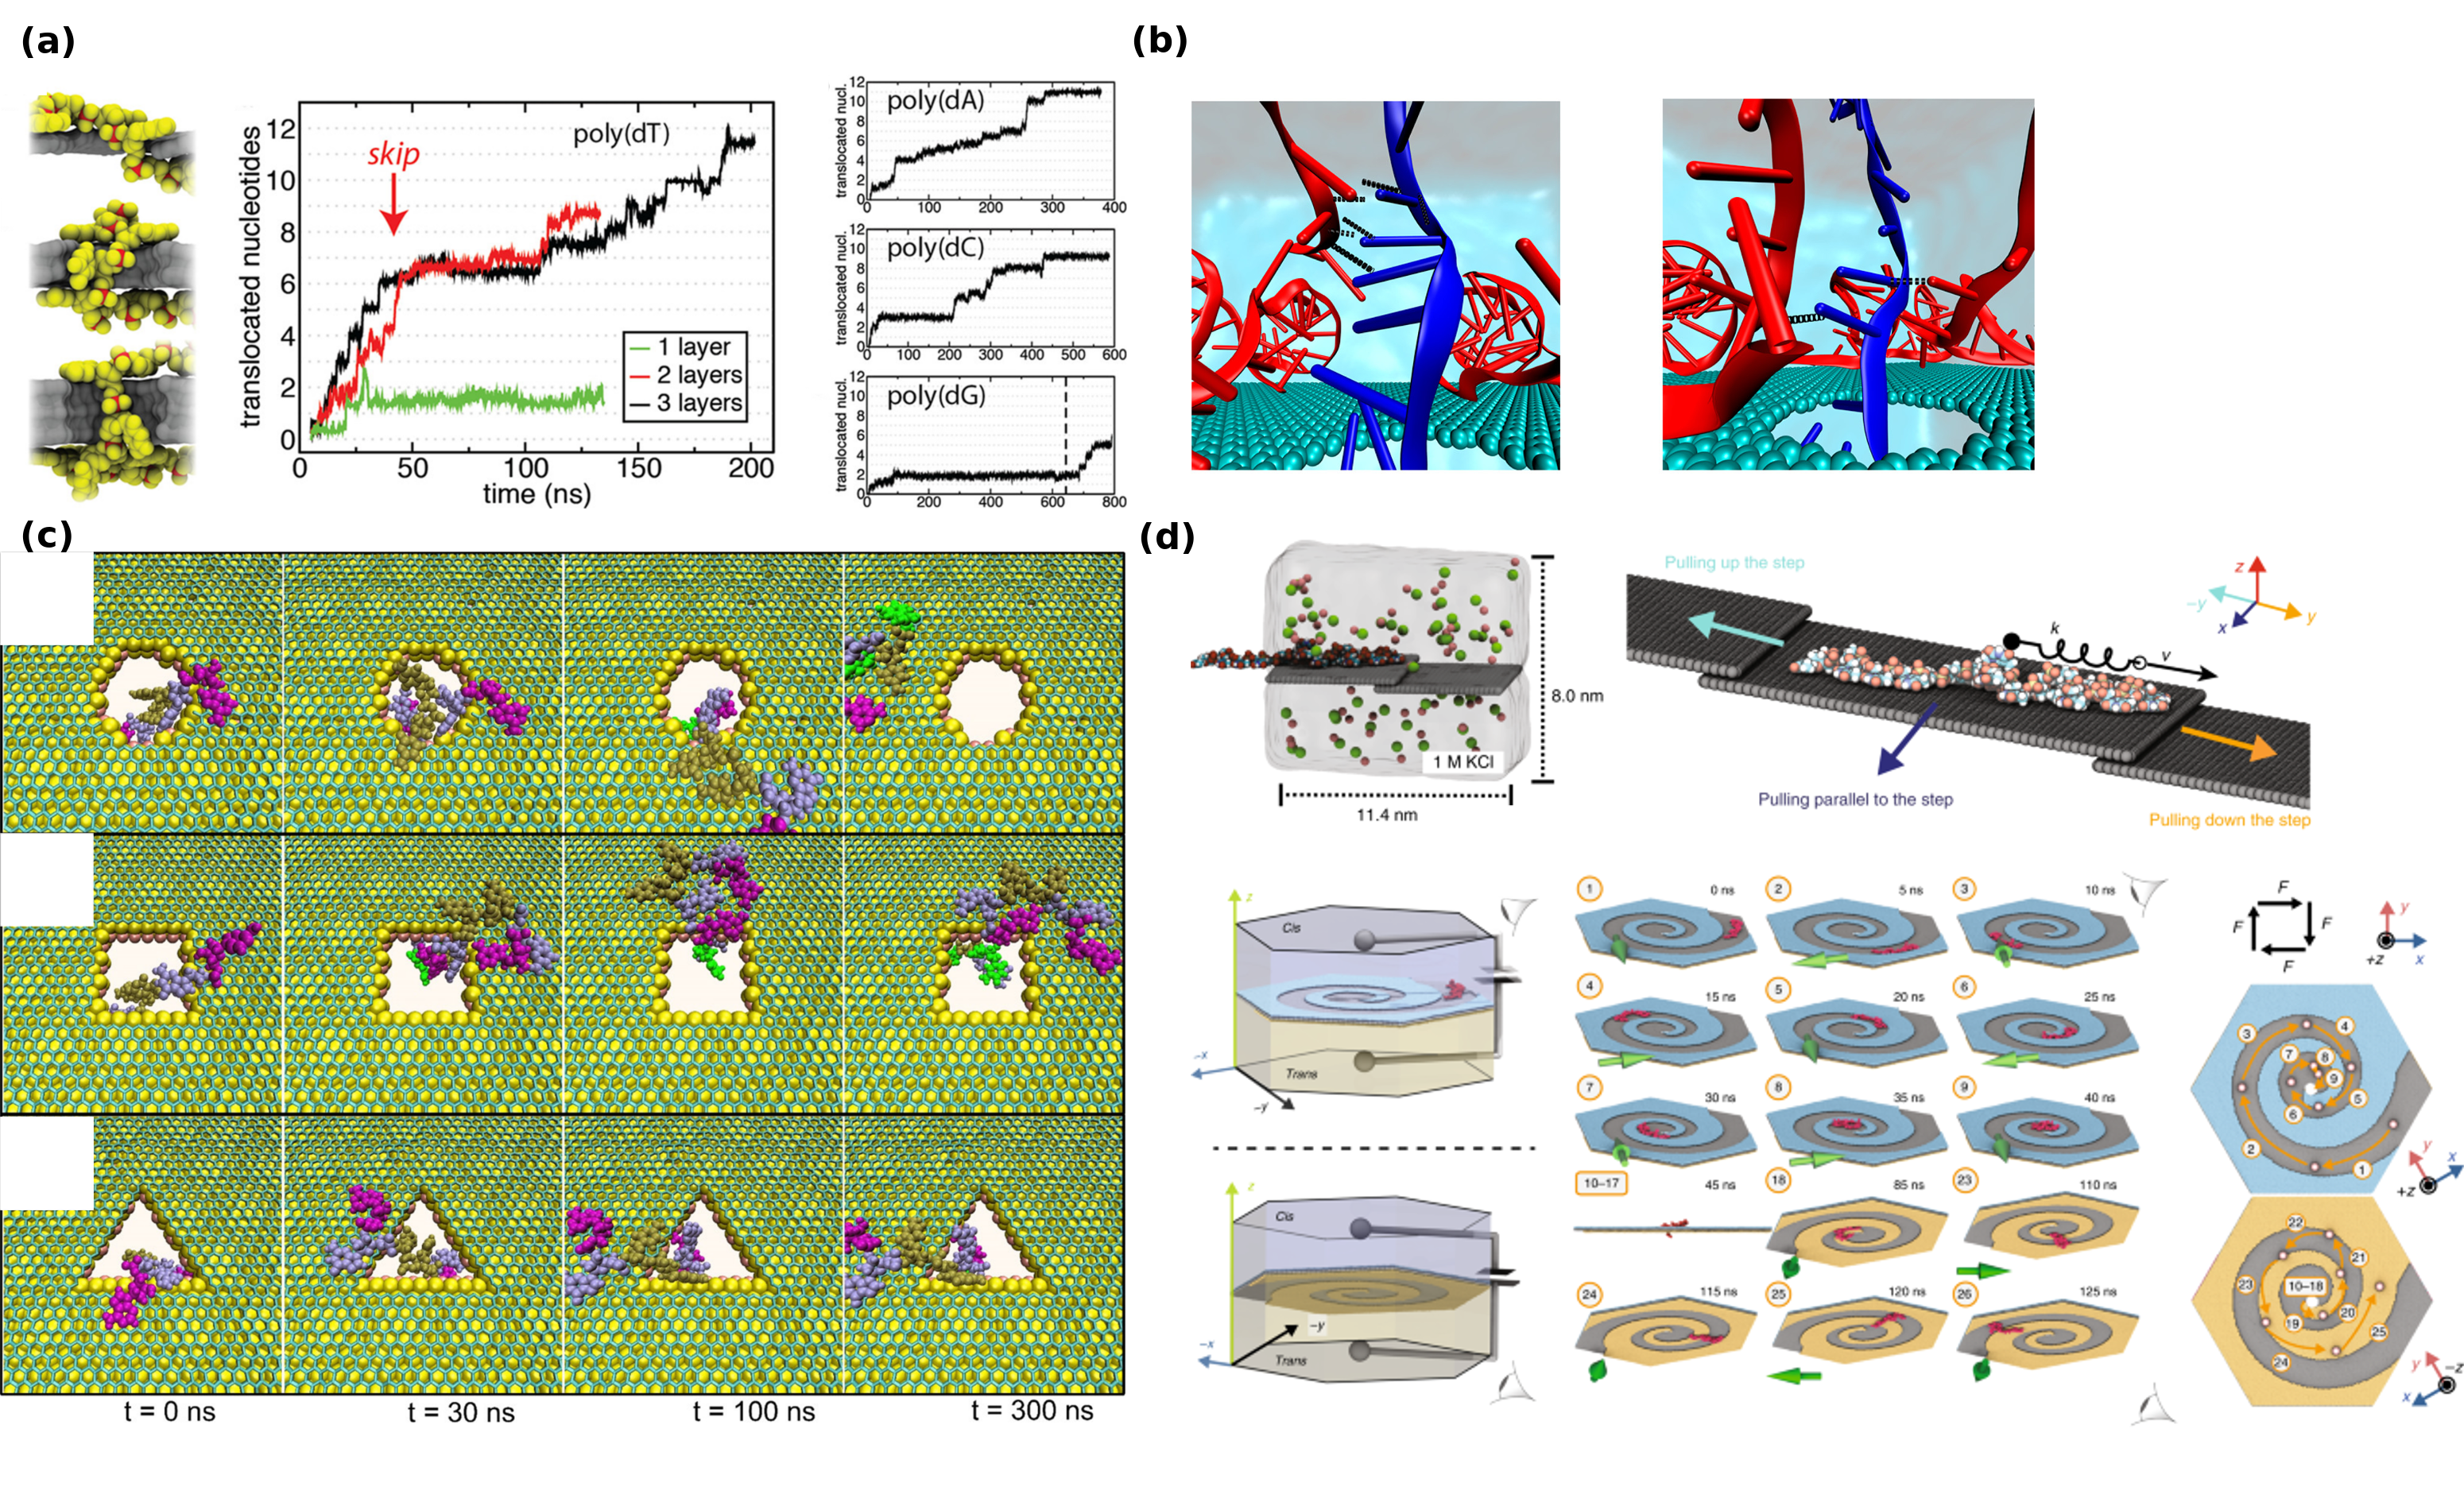
\includegraphics[width=\textwidth]{Introduction/Figures/figure_ssDNA_sim}
    \caption[Results from ssDNA - graphene nanopore all-atom MD simulations]{(a) Representative figures depicting the system setup and progress of translocations of ssDNA through nanopores of varying thicknesses. (b) Hydrogen bonds between poly(dA) and poly(dT) with DNA origami. (c) Representative snapshots of translocated nucleotides of ssDNA in circular, square and triangular graphene–MoS\textsubscript{2} heterostructure nanopores.  (d) Representaive images depicting the three pulling directions investigated and the motion of ssDNA along the defect channels under an applied external force. Panel (a) reprinted (adapted) from ref \supercite{wells_assessing_2012}. Copyright 2023 American Chemical Society. Panel(b) reprinted (adapted) with permission from ref \supercite{barati_farimani_dna_2017}. Copyright 2023 American Chemical Society. Panel (c) reprinted (adapted) with permission from ref \supercite{zou_spontaneous_2020}. Copyright 2023 American Chemical Society. Panel (d) reprinted (adapted) with permission from ref.\supercite{shankla_step-defect_2019}. Copyright 2023 Nature Publishing Group.}
    \label{fig:figure16}
\end{figure}

Using all-atom MD simulations, Aksimenteiv and colleagues demonstrated that few-layer graphene membranes can act as suitable tools for rapid and accurate sequencing of ssDNA.\supercite{wells_assessing_2012} They investigated the translocation dynamics of four ssDNA homopolymers (adenine, guanine, cytosine and thymine) through multiple pore geometries and membranes of various thicknesses using non-polarizable additive FF simulations [Figure 1.16(a)]. They demonstrated that the interactions between the graphene surface and the ssDNA strand could significantly slow the transport of ssDNA across the graphene membrane. They noted that the transport of ssDNA across the graphene membrane occurs in single nucleotide steps. However, they also noted that the transport mechanism does not proceed in one direction leading to multiple entries and exits being registered for a single nucleotide, eventually leading to an erroneous readout of the ssDNA sequence.

Aluru and coworkers employed all-atom MD simulations to evaluate the translocation dynamics of an ssDNA through a DNA origami-decorated graphene nanopore.\supercite{barati_farimani_dna_2017} They employed a modified DNA strand with eight adenine nucleotides removed from the template strand, leaving eight free thymine nucleotides of the complementary strand as a decorator over the nanopore. They observed that at a particular voltage, the transport of the ssDNA across the hybrid nanopore depends on the interactions between the ssDNA and the DNA origami, with the dwell time of $\sim$ 3 ns for polydA, due to its interaction with the complementary T nucleotides in the DNA origami [Figure 1.16(b)]. Even though DNA origami only had free T nucleotides, the formation of hydrogen bonds between the polydC strand and the G-C base pairs in the DNA origami led to a significant dwell time for polydC strands. From ionic current measurements, they demonstrated that ionic current measurements could reliably identify A and G bases, while T and C bases have similar ionic currents. The authors opined that a statistical analysis of ionic current and dwell times could reliably identify the four bases.

Zhou and colleagues investigated the effect of various pore geometries in a graphene-MoS\textsubscript{2} heterostructure on the spontaneous transport of ssDNA across the membrane, using MD simulations\supercite{zou_spontaneous_2020}. They observed significantly slower translocations in triangular nanopores, while the translocations were observed to be the fastest in circular nanopores [Figure 1.16(c)]. Their observations of the spontaneous transport of ssDNA across the heterostructure were rationalised using the electrostatic interactions between the positively charged Mo ions and the negatively charged phosphate (PO\textsubscript{4}\textsuperscript{-}) groups in the ssDNA. This observation of spontaneous transport of ssDNA under the influence of chemical potential, and without an explicit applied external bias is in line with the previous observations by Zhou and coworkers, where a similar transport was observed from MD simulations\supercite{luan_spontaneous_2018}.

Shankla and Aksimenteiv investigated the motion of an ssDNA along a step-defect using all-atom MD simulations\supercite{shankla_step-defect_2019}. Using constant velocity-steered MD (SMD) simulations, the authors demonstrated a sharp increase in the force acting on the ssDNA molecules at a defect junction, which quickly drops to zero once the molecule has crossed the junction. They also noted a directional dependence on the force, with a higher force ($\approx$ 2-2.5 times) required to pull the ssDNA up a defect junction than to move it down a defect junction. The authors reasoned that the origin of this difference could be attributed to the hydration of the nucleotide, with the nucleotide losing the hydration as it moves up the defect junction and then getting rehydrated once it moves past the junction. In contrast, while the nucleotide moves down the defect junction, it first gains hydration, which is then lost as it moves across the junction, and finally regains the hydration as it moves past the defect junction. The authors also demonstrated that a step-guided pattern that transport ssDNA either towards or away from a nanopore [Figure 1.17(d)]. 

Shankla and Aksimenteiv employed all-atom MD simulations to also study the translocation dynamics of an ssDNA through a charged graphene nanopore\supercite{shankla_conformational_2014}. The authors used a poly-dT\textsubscript{20} strand to model an ssDNA and investigated the dynamics of the ssDNA through three nanopores, where the graphene sheets had a surface charge density between -2 and 2e/nm\textsuperscript{2} in steps of 0.5. They observed that the charge of the graphene sheet has a significant effect on the dynamics of the ssDNA, with the interactions between the ssDNA and the graphene surface being drastically different between -2e/nm\textsuperscript{2} and 2e/nm\textsuperscript{2} simulations. For a charge-neutral system (0e/nm\textsuperscript{2}), they observed that the strand has significant interactions with the graphene sheet via stacking interactions between the nucleobases and the surface. At the same time, the negatively charged phosphate groups did not interact with the surface. However, upon increasing the charge to +2e/nm\textsuperscript{2}, they observed that the nucleobases' orientation had changed to 47$\degree$ from 0$\degree$, indicating that the negatively charged phosphate groups had started interacting with the positively charged graphene surface. On a similar footing, changing the surface charge density to -2e/nm\textsuperscript{2} has the opposite effect, where the ssDNA would be repelled away from the graphene surface. The authors observed that these interactions are reversible, meaning it is possible to convert from one state to another by changing the surface charge density on the graphene surface. For other homopolymers considered in the study (dA\textsubscript{20}, dG\textsubscript{20}, dC\textsubscript{20} and a methylated version of dC\textsubscript{20}), very similar dynamics were observed where some or all nucleobases were observed to be repelled away from the surface at a surface charge density of -2e/nm\textsuperscript{2}. However, they observed different dynamics at the other end of the surface charge density (2e/nm\textsuperscript{2}), where some combination of orientations (flat, tilted and unbound) were observed for the four homopolymer strands. To comment on the effect of surface charge density on the translocation of ssDNA through the nanopore, the authors investigated the translocation of ssDNA through the same nanopores at an applied external bias of 500 mV. They observed that the translocation velocity of the dT\textsubscript{20} strand depended on the surface charge density, with the translocation velocity varying in a correlated manner with the surface charge density. As a proof-of-concept, the authors also demonstrated a stop-and-go type of dynamics for the ssDNA by changing the surface charge densities and the applied external bias, where they demonstrated that under a constant applied external bias, changing the surface charge density would halt the translocation of the ssDNA through the nanopore.  

Smolyanitsky and coworkers employed all-atom MD simulations to investigate the applicability of a cytosine-decorated graphene nanopore as a functional material for DNA sequencing.\supercite{paulechka_nucleobase-functionalized_2016} They studied the efficacy of the functionalized nanopore in detecting guanine nucleobases present in the ssDNA strand by using the ripples generated in the graphene nanoribbon (GNR) during the translocation of ssDNA. They demonstrated that a cytosine-functionalized nanopore could reliably identify guanine-rich segments in the translocating ssDNA.

Schulten and coworkers investigated the translocation dynamics of poly-dA\textsubscript{14} through a nanopore constructed in a graphene nanoribbon using steered molecular dynamics (SMD) simulations\supercite{qiu_intrinsic_2015}. They observed that the ssDNA would undergo quicker translocations if the 3'-end of the ssDNA is threaded through the nanopore, in contrast to the 5'-end where the translocations were more sluggish, giving rise to the step-wise translocations previously reported in the literature.  They reasoned that by reversing the pulling direction inorder to translocate the 3' end of the ssDNA through the nanopore, the DNA bases can form a bigger angle with the graphene surface normal and, can move quicker through the nanopore; while pulling in the original direction, with the 5'-end translocating first, the DNA bases would form a smaller angle with the graphene surface, increasing the probability of the nucleobases getting stuck in the nanopore, giving rise to stepwise translocations.

\section{Conclusions}
Here, we have summarised a few critical experimental and computational investigations demonstrating the applications of graphene as a solid-state support for 2D SAM formation and a solid-state membrane for rapid and accurate DNA sequencing. These research studies underline the importance of graphene and (or) graphene-like materials as solid-state support and functional materials for biological applications. The electronic structure of graphene can be tuned based on the electronic nature of the adsorbed molecules, opening up the possibility of using graphene as a functional material for sensing applications. However, we note that MD simulations based on classical additive FFs need further improvement in describing the formation of such self-assemblies\supercite{saikia_hierarchical_2017,saikia_dynamics_2018}. Few authors investigated the development of FFs specifically parameterized to describe such interactions, but they are generally not transferable between systems\supercite{manukyan_first_2015}. Previous studies based on ab-inito calculations have demonstrated that the strength of the non-covalent interactions between the nucleobases and the underlying graphene surface is proportional to the molecular polarizability of the nucleobases and the surface.\supercite{gowtham_physisorption_2007} However, additive non-polarizable FF simulations, based on fixed point charges are unable to describe molecular polarizability, leading to errenous simulation outcomes. This indicates that a polarizable description for all the components is a necessary requirement towards understanding the self-assembly of nucleobases and (or) other small molecules at the graphene interface.  

The outbreak of the severe acute respiratory syndrome coronavirus 2 (Sars-Cov-2) and the swift progress in the development of treatment protocols hightlights the need for a fast, reliable and afforable method for DNA sequencing. In this context, graphene nanopores have emerged as a suitable material for DNA sequencing. Multiple authors have investigated various methodologies for efficiently using graphene membranes as a DNA sequencing tool. We want to highlight the work by Aksimenteiv and coworkers, where they demonstrated that two channels of opposite chirality can transport ssDNA across the nanopore without pore clogging\supercite{shankla_step-defect_2019}. Those simulations were performed using additive FF, and further investigations using classical Drude FF might be required to further understand ssDNA's transport across the nanopore. We note that investigations about the specific effects of water and ions on the transport of DNA strands across the graphene membranes and their effects on the ionic and (or) transverse current measurements still need to be explored.

To this end, ionic conductivity and transport phenomena in nanopores, nanochannels is an active field of investigation with better representations required to capture the associated dynamics. Some recent developments to this end have been the use of non-equilibrium modelling to capture the concentration dependent dynamics.\supercite{nazari_transport_2020,karmakar_non-equilibrium_2023} Recent experimental studies have explored transverse detection of DNA strands using both graphene\supercite{heerema_probing_2018} and MoS\textsubscript{2} nanopores,\supercite{graf_transverse_2019} wherein nucleobase detection was observed in both the cases. Theoretically many groups have explored transverse current signatures of nucleobases trapped within a nanopore, however a limitation with this work is that these DFT bases calculations are performed using single layer nanopores.\supercite{prasongkit_transverse_2011,lagerqvist_fast_2006,prasongkit_theoretical_2015} A multilayer description must be adopted for a better description of nanopore interactions as evidenced by simulation studies.\supercite{wells_assessing_2012} We expect to see more investigations from both experimental and theoretical point of views aimed at investigating the transport of DNA molecules across nanopores.

\section{Thesis Objectives}
The overall objective of this thesis is to provide a generalized methodology to investigate the dynamics of small molecules in presence of a graphene surface. The specific objectives are:
\begin{itemize}
    \item To transfer and test the Drude polarizable FF parameters to describe a polarizable graphene sheet, and to investigate the dynamics of nucleobases in the presence of a polarizable graphene surface.
    \item To investigate the dynamics of mono and divalent ions in the presence of a graphene surface, to gain insights on the interaction patterns of the ions with the graphene surface.
    \item To investigate the dynamics of a ssDNA translocating through a pristine graphene nanopore, to gain insights into the experimentally observed pore clogging, and to gain insights into the various factors that affect the translocation dynamics. 
\end{itemize}

\section{Thesis Outline}
 Using all-atom MD simulations, in conjunction with Drude polarizable FF parameterization, we investigate the dynamics of nucleobases, ions and short ssDNA strands in presence of a polarizable graphene surface to gain a critical understanding of the interfacial dynamics. In this section, we provide a brief overview of the thesis. This thesis is divided into six chapters, with a brief description of each chapter provided here.

\begin{itemize}
    \item \textbf{Chapter 1} provides a survey of the literature pertaining to the applications of graphene and (or) graphite in the domains of nucleobase self-assemblies and as functional materials for DNA sequencing. 
    \item \textbf{Chapter 2} provides a brief overview of the simulation methods used in this thesis and also provides a summary of Adaptive Biasing Force simulations.
    \item \textbf{Chapter 3} reports the development of Drude polarizable FF paraneters for graphene, and the effect of molecular polarizability on the dynamics of nucleobases disperesed over a graphene surface.
    \item In \textbf{Chapter 4}, polarizable force field simulations elucidate the aggregation behaviour of nucleobases on a graphene surface as a function of solute concentration, providing valuable insights into their dynamics.
    \item In \textbf{Chapter 5}, polarizable force field simulations elucidate the dynamics of electrolyte solutions in close contact with a polarizable graphene surface. We also report an accurate reproduction of the ion-graphene interactions from polarizable simulations.  
    \item \textbf{Chapter 6} provides an atomistic description of the factors influencing the translocation dynamics of a single-stranded DNA (ssDNA) as it moves through a pristine graphene nanopore.
\end{itemize}

\section{List of Publications}
\begin{itemize}
    \item \textbf{H., Hemanth} and Mallajosyula*, S.S.; Polarization Influences the Evolution of Nucleobase - Graphene Interactions; {\textit{Nanoscale}, 2021, \textbf{13}, 4060 - 4072}
    \item \textbf{H., Hemanth}, Yadav, P. K. and Mallajosyula*, S.S.; Capturing Concentration Induced Aggregation of Nucleobases on Graphene Surface Through Polarizable Forcefield Simulations; {\textit{J. Phys. Chem. C}, 2022, \textbf{31}, 13122 - 13131}
    \item \textbf{H., Hemanth}, Mewada, R. and Mallajosyula*, S.S.; Capturing Charge and Size Effects of Ions at the Graphene - Electrolyte Interface Using Polarizable Force Field Simulations; {\textit{Nanoscale Adv.}, 2023, \textbf{5}, 796 - 804}
    \item \textbf{H., Hemanth} and Mallajosyula*, S.S.; Unveiling DNA Translocation in Pristine Graphene Nanopores: Understanding Pore Clogging via Polarizable Simulations; {\textit{ACS Appl. Mater. Interfaces}, 2023, \textbf{47}, 55095-55108} 
    \item \textbf{H., Hemanth} and Mallajosyula*, S.S.; Graphene: From Solid Support for Nucleobase Assisted Self-Assemblies to Functional Material for DNA Sequencing \textit{(Accepted for publication at J. Phys. Chem. C)} 
\end{itemize}
